\documentclass[9pt,twocolumn,twoside]{pnas-new}
% Use the lineno option to display guide line numbers if required.
% Note that the use of elements such as single-column equations
% may affect the guide line number alignment. 

\templatetype{pnasresearcharticle} % Choose template 
% {pnasresearcharticle} = Template for a two-column research article
% {pnasmathematics} = Template for a one-column mathematics article
% {pnasinvited} = Template for a PNAS invited submission

% added to enable supplementary figures
\usepackage{placeins}
\usepackage{newfloat}
\DeclareFloatingEnvironment[name={Figure}]{suppfigure}
\renewcommand{\thesuppfigure}{S\arabic{suppfigure}}

\DeclareFloatingEnvironment[name={Dataset}]{suppdata}
\renewcommand{\thesuppdata}{S\arabic{suppdata}}

\newcommand{\comment}[1]{{\color{red}[\textsl{#1}]}}

\title{Deep mutational scanning of hemagglutinin helps distinguish the evolutionary fate of human H3N2 influenza virus lineages}

% Use letters for affiliations, numbers to show equal authorship (if applicable) and to indicate the corresponding author
\author[a,d,e,1]{Juhye M. Lee}
\author[b,f,1]{John Huddleston} 
\author[a,d,e]{Michael B. Doud}
\author[a,f]{Kathryn A. Hooper}
\author[b,c,2]{Trevor Bedford}
\author[a,c,d,2]{Jesse D. Bloom}

\affil[a]{Basic Sciences Division}
\affil[b]{Vaccine and Infectious Diseases Division}
\affil[c]{and Computational Biology Program, Fred Hutchinson Cancer Research Center, Seattle, WA 98109, USA}
\affil[d]{Department of Genome Sciences}
\affil[e]{Medical Scientist Training Program}
\affil[f]{and Molecular and Cellular Biology Program, University of Washington, Seattle, WA 98195, USA}

% Please give the surname of the lead author for the running footer
\leadauthor{Lee} 

% Please add here a significance statement to explain the relevance of your work
% 120 words max
\significancestatement{
Mutations drive the rapid evolution of seasonal influenza virus such that new strains emerge and co-circulate until one strain overtakes the population. 
A key challenge in the study of seasonal influenza virus is to be able to differentiate between strains that are likely to persist and those that are likely to die out. 
We therefore need a greater understanding of how mutations drive and constrain viral evolution in order to help identify persistent and nonpersistent strains. 
We experimentally measured the effect of every possible amino-acid mutation to the surface protein hemagglutinin on viral growth.
Using these measurements, we revealed differences between successful and unsuccessful viral lineages and examined how generalizable the measurements were for studying the evolutionary fate of viral lineages.
\comment{Our work has potential for use in forecasting}
}

% Please include corresponding author, author contribution and author declaration information
\authorcontributions{Please provide details of author contributions here.}
\authordeclaration{Please declare any conflict of interest here.}
\equalauthors{\textsuperscript{1}J.M.L. and J.H. contributed equally to this work.}
\correspondingauthor{\textsuperscript{2}To whom correspondence should be addressed: trevor@bedford.io, jbloom@fredhutch.org}

% Keywords are not mandatory, but authors are strongly encouraged to provide them. If provided, please include two to five keywords, separated by the pipe symbol, e.g:
\keywords{influenza virus $|$ hemagglutinin $|$ deep mutational scanning $|$ antigenic drift $|$ epistasis} 

\begin{abstract}
% no more than 250 words. (199 now)
The evolution of seasonal H3N2 influenza virus is mediated by the rapid accumulation of mutations. 
A better understanding of how mutations affect viral growth is critical for studying the pressures and constraints underlying the evolution of the influenza virus in nature. 
Here we experimentally measure the effect of every possible single amino-acid mutation to an H3 influenza hemagglutinin on viral growth in cell culture. 
We find the stalk domain to be fairly mutationally tolerant, and there is not a large disparity in tolerance between the head and stalk domains.
Furthermore, our measurements reveal mutations in successful seasonal influenza viral lineages to be significantly more preferred than mutations in lineages that have died out, and this was true at both epitope and non-epitope sites.
Epistasis in hemagglutinin is also seemingly driven by antigenic drift.
The preferences measured in a distantly related protein homolog do not reveal such differences in viral lineages.
A comparison of the preferences between the two hemagglutinin variants show substantial shifts in the effects of mutations.
Overall, our work highlights how experimental measurements of mutational effects can be leveraged to gain insight into the evolutionary fates of viral strains and potentially be used to predict viral evolution.
\end{abstract}

\dates{This manuscript was compiled on \today}
\doi{\url{www.pnas.org/cgi/doi/10.1073/pnas.XXXXXXXXXX}}

\begin{document}

% Optional adjustment to line up main text (after abstract) of first page with line numbers, when using both lineno and twocolumn options.
% You should only change this length when you've finalised the article contents.
\verticaladjustment{-2pt}

\maketitle
\thispagestyle{firststyle}
\ifthenelse{\boolean{shortarticle}}{\ifthenelse{\boolean{singlecolumn}}{\abscontentformatted}{\abscontent}}{}

\dropcap{S}easonal H3N2 influenza virus evolves rapidly, fixing 3 to 4 amino-acid mutations per year in its hemagglutinin (HA) surface protein.
 Many of these mutations contribute to the rapid antigenic drift that necessitates frequent updates to the annual influenza vaccine~\cite{smith2004mapping,bhatt2011genomic}.
This evolution is further characterized by strain competition and frequent population turnover~\cite{fitch1997long,strelkowa2012clonal,bedford2011,neher2014predicting,koelle2015effects,bedford2015global}, producing a spindly phylogenetic tree with a persistent trunk lineage and short-lived side branches~\cite{fitch1991positive} (Figure~\ref{fig:H3N2_phylogeny}).
Several lines of evidence indicate that the trunk lineage outcompetes other strains at least in part because it has higher fitness~\cite{strelkowa2012clonal,bedford2011,neher2014predicting,koelle2015effects}.
A key challenge in the study of H3N2 evolution is to forecast which strain will dominate the upcoming influenza season, as this information can guide selection of a vaccine strain~\cite{morris2017predictive}.
In order to make these forecasts, it is important to identify the features that enable the trunk strain to persist as other strains die out.

\begin{figure}
\centering
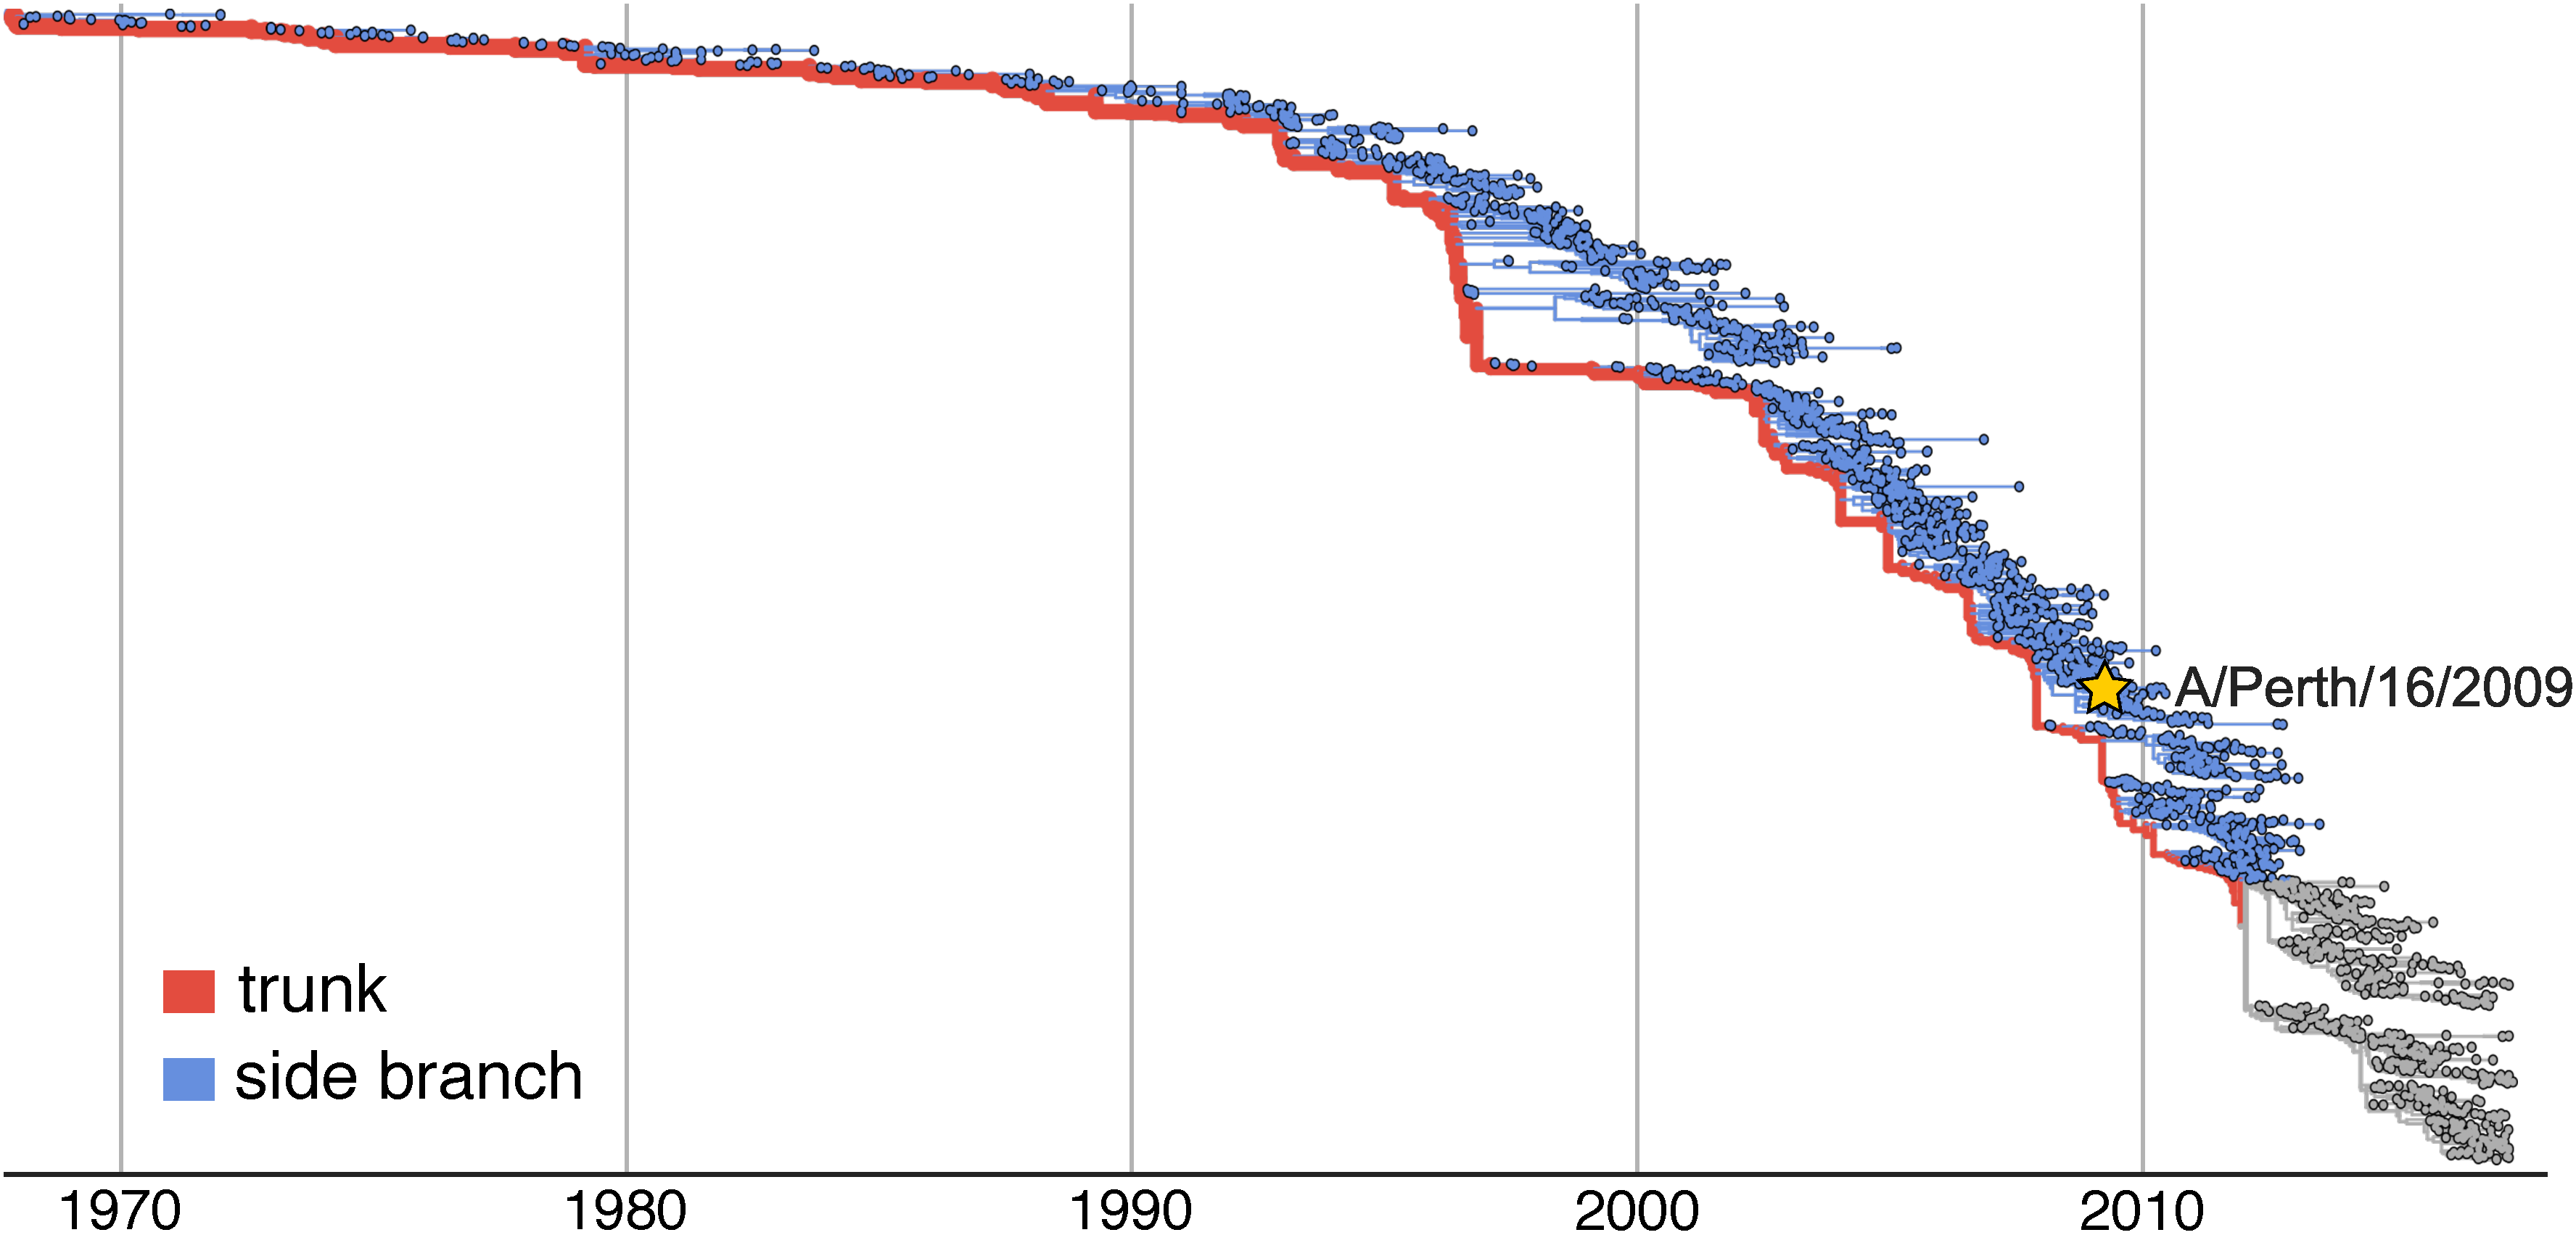
\includegraphics[width=\linewidth]{figs/H3N2_phylogeny/H3N2_phylogeny.pdf}
\caption{\label{fig:H3N2_phylogeny}
{\bf Human H3N2 HA phylogeny from 1968-2017.}
The trunk is shown in red, and side branches are shown in blue.
The gray branches represent the part of the tree for which we cannot yet distinguish the trunk from side branches.
The Perth/2009 strain is indicated with a star.
}
\end{figure}

%To aid in the timeliness and throughput of making such decisions, previous work have endeavored to accurately predict the evolutionary outcomes of viral strains based on the antigenicity and/or tree structure of viral clades~\cite{steinbruck2014computational,neher2014predicting}.
%However, the accuracy of these predictions are subject to uneven geographical and temporal sampling, and for~\cite{neher2014predicting}, the lack of information about a mutation's effect on antigenicity.

Two main features distinguish the evolutionarily successful trunk from its competitors: greater antigenic change, and efficient viral growth and transmission.
In principle, experiments could be informative for identifying how mutations affect these features.
Most work on influenza evolution to date has utilized experimental data primarily to assess the antigenicity of circulating strains~\cite{sun2013using,harvey2016identification,neher2016prediction}.
While the antigenic features of a virus certainly contribute to its success, the non-antigenic effects of mutations also play an important role~\cite{pybus2007phylogenetic,kucharski2011influenza,strelkowa2012clonal,luksza2014predictive,koelle2015effects}.
Specifically, due to influenza virus's high mutation rate~\cite{holland1982rapid,steinhauer1987rapid,lauring2010quasispecies} and lack of intra-segment recombination~\cite{boni2008homologous}, deleterious mutations become linked to beneficial ones.
The resulting accumulation of deleterious mutations can affect non-antigenic properties that are central to viral fitness~\cite{luksza2014predictive}.
However, while extensive work has gone into characterizing how mutations affect HA antigenicity~\comment{epitope site papers, Koel paper, Hensley papers, Kawaoka paper}, we lack any large-scale quantitative characterization of how mutations to H3N2 HA affect non-antigenic properties crucial to viral fitness.

It is now possible to use deep mutational scanning~\cite{fowler2014deep} to measure the functional effects of large numbers of mutations to viral proteins~\cite{thyagarajan2014inherent,wu2014high,doud2016accurate,haddox2016experimental,qi2015high}.
However, the only HA for which so such measurements have previously been made is from the highly lab-adapted A/WSN/1933 (H1N1) strain~\cite{thyagarajan2014inherent,wu2014high,doud2016accurate}.
Here we measure the effects on viral growth in cell culture of all mutations to the HA from a recent human H3N2 strain, A/Perth/16/2009.
We then examine whether these measurements are useful for distinguishing between H3N2 trunk and side branch lineages, and find that mutations on the trunk are measured to be more favorable than those on the side branches, both at epitope and non-epitope sites.
However, the experiments are useful for assessing the effects of mutations only in closely related viral strains, since we show that mutations often have disparate effects on H3 and H1 HAs.
Our work highlights the potential for using high-throughput experimental measurements of mutational effects to inform evolutionary forecasting of human seasonal influenza virus.

\section*{Results}
\label{sec:results}

\subsection*{Deep mutational scanning of HA from a recent strain of human H3N2 influenza virus}
We performed a deep mutational scan to measure the effects of all amino-acid mutations to HA from the A/Perth/16/2009 (H3N2) strain on viral replication in cell culture. 
This strain was the H3N2 component of the influenza vaccine from 2010-2012~\cite{who2010d,who2011}.
Relative to the consensus sequence for this HA in Genbank, we used a variant with two mutations that enhanced viral replication in cell culture, G78D and T212I (Figure~\ref{suppfig:Perth2009_mut} and Dataset~\ref{suppdata:PerthHA}).
The G78D mutation occurs at low frequency in natural H3N2 sequences, and T212 is a site where a mutation to Ala rose to fixation in human influenza in $\sim$2011.

We mutagenized the entire HA coding sequence at the codon level to create mutant plasmid libraries harboring an average of $\sim$1.4 codon mutations per clone (Figure~\ref{suppfig:SangerSeq}).
We then generated mutant virus libraries from the mutant plasmids using a helper-virus system that enables the efficient generation of complex influenza virus libraries~\cite{doud2016accurate} (Figure~\ref{fig:dms_overview}A).
These mutant viruses derived all their non-HA genes from the lab-adapted A/WSN/1933 strain.
Using WSN/1933 for the non-HA genes reduces biosafety concerns, and also helped increase viral titers.
To further increase viral titers, we used MDCK-SIAT1 cells that we had engineered to constitutively express the TMPRSS2 protease, which facilitates HA cleavage and activation~\cite{bottcher2006proteolytic, bottcher2010cleavage}.

\begin{SCfigure*}[\sidecaptionrelwidth][t]
\centering
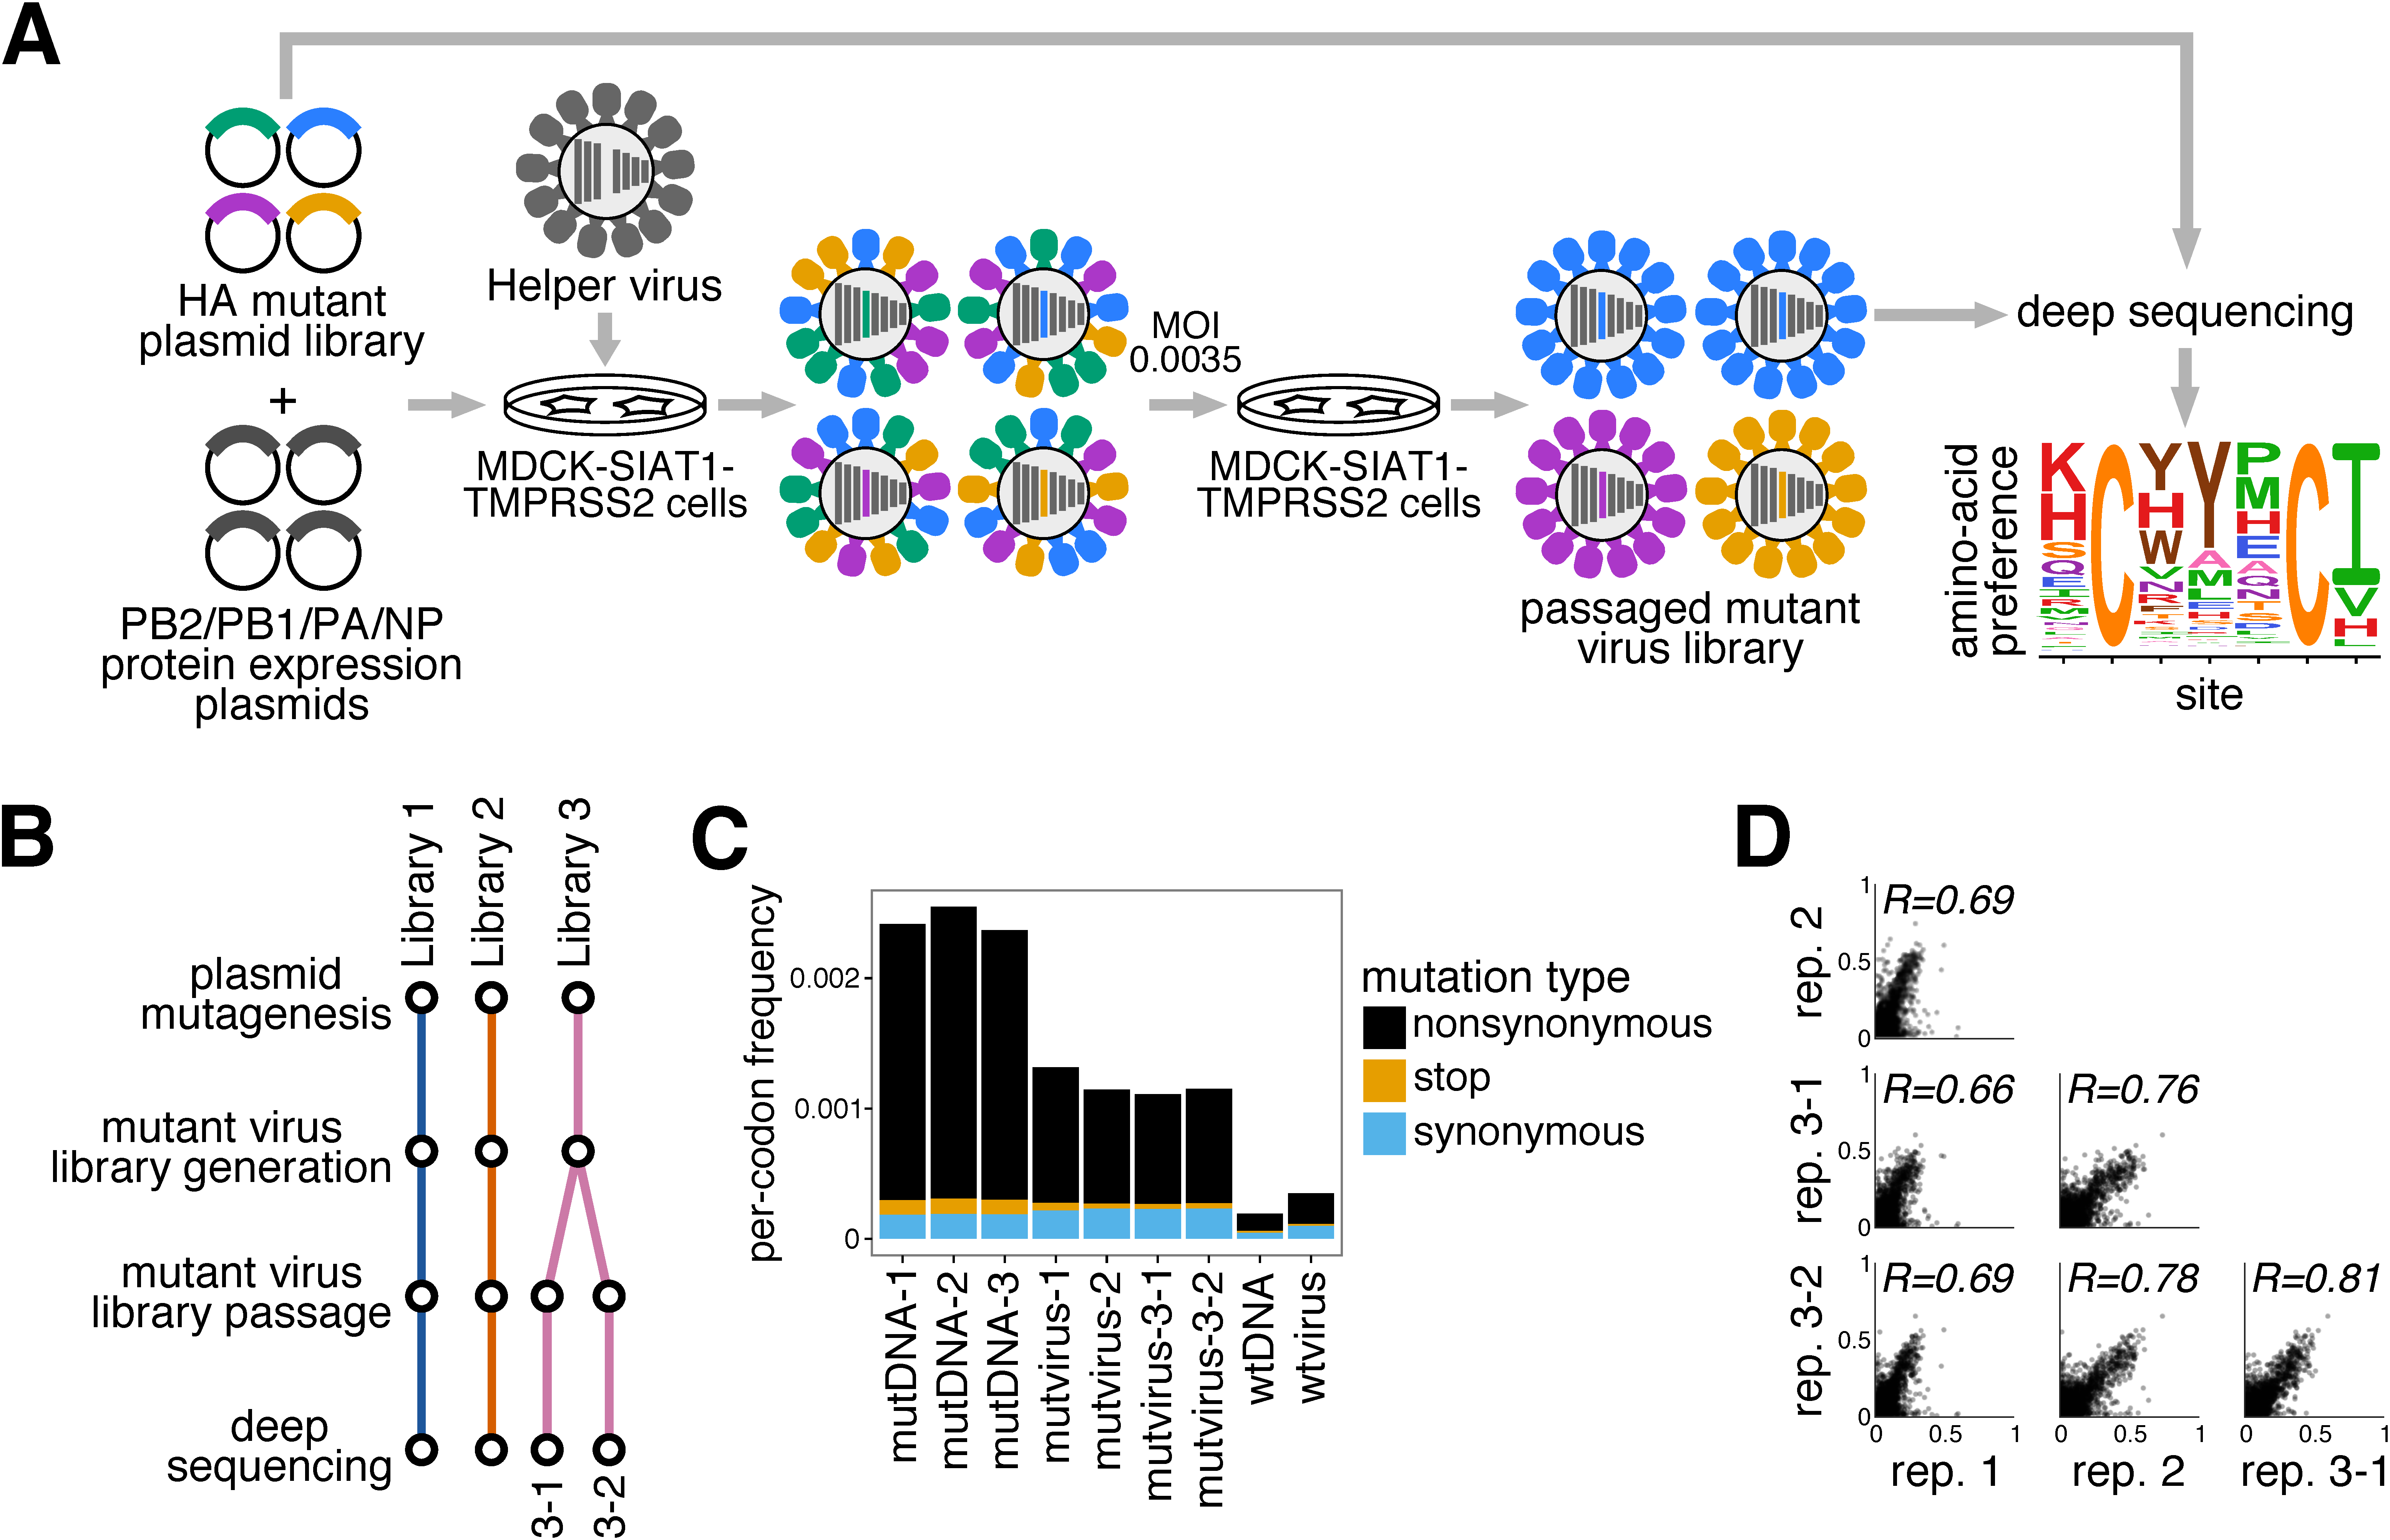
\includegraphics[width=12cm]{figs/dms_overview/dms_overview.pdf}
\caption{\label{fig:dms_overview}
{\bf Deep mutational scanning of the Perth/2009 H3 HA.}
(A) We generated mutant virus libraries using a helper-virus approach~\cite{doud2016accurate}, and passaged the libraries at low MOI to establish a genotype-phenotype linkage and to select for functional HA variants. 
Deep sequencing of the variants before and after selection allowed us to estimate each site's amino-acid preferences.
(B) The experiments were performed in full biological triplicate. 
We also passaged and deep sequenced library 3 in duplicate.
(C) Frequencies of nonsynonymous, stop, and synonymous mutations in the mutant plasmid DNA, the passaged mutant viruses, and wildtype DNA and virus controls. 
(D) The Pearson correlations among the amino-acid preferences estimated in each replicate. 
}
\end{SCfigure*}

After generating the mutant virus libraries, we passaged them at low MOI in cell culture to create a genotype-phenotype link and select for functional HA variants (Figure~\ref{fig:dms_overview}A).
All the experiments were completed in full biological triplicate (Figure~\ref{fig:dms_overview}B). 
We also passaged and deep sequenced library 3 in duplicate (denoted as library 3-1 and 3-2) to gauge the experimental noise occurring \textit{within} a single biological replicate.
As a control to measure sequencing and mutational errors, we used the unmutated HA gene to generate and passage viruses carrying wildtype HA.

Deep sequencing of the initial plasmid mutant libraries and the passaged mutant viruses revealed selection for functional HA mutants.
Specifically, stop codons were purged to 20-45\% of their initial frequencies after correcting for error rates estimated by sequencing the wildtype controls (Figure~\ref{fig:dms_overview}C).
The incomplete purging of stop codons is likely because genetic complementation due to co-infection~\cite{marshall2013influenza} enabled the persistence of some virions with nonfunctional HAs. 
We also observed selection against many nonsynonymous mutations (Figure~\ref{fig:dms_overview}C), with their frequencies falling to 30-40\% of their initial values after error correction.

We next quantified the reproducibility of our deep mutational scanning measurements across biological and technical replicates. 
We first used the deep sequencing data for each replicate estimate the preference of each site in HA for all 20 amino acids using the method described in~\cite{bloom2015software}.
Because there are 567 residues in HA, there are $567 \times 20 = 11,340$ estimated amino-acid preferences.
The correlations of the amino-acid preferences between pairs of replicates are shown in Figure~\ref{fig:dms_overview}D.
The biological replicates are fairly well-correlated, with Pearson's $R$ ranging from 0.69 to 0.78. 
Replicate 1 exhibited the lowest correlation with the other replicates; this replicate also showed the weakest selection against stop and nonsynonymous mutations (Figure~\ref{fig:dms_overview}C), perhaps indicating more experimental noise.
The two technical replicates 3-1 and 3-2 were only slightly more correlated than pairs of biological replicates, suggesting that bottlenecking of library diversity after the reverse-genetics step contributes most of the experimental noise.

\subsection*{Our measurements are consistent with existing knowledge about HA's evolution and function}
How do the HA amino-acid preferences measured in our experiments relate to the evolution of H3N2 influenza virus in nature?
This question can be addressed by evaluating how well an experimentally informed codon substitution model (ExpCM) using our measurements describe H3N2 evolution compared to standard phylogenetic substitution models~\cite{bloom2017identification,hilton2017phydms}.
Table~\ref{tab:phydms} shows that the ExpCM using the across-replicate average of our measurements greatly outperforms conventional substitution models.
This result indicates that our experiments authentically capture some of the constraints on HA evolution. 
The relative rate of nonsynonymous to synonymous substitutions (dN/dS or $\omega$) is $\ll$1 for conventional substitution models.
However, the relative rate of nonsynonymous to synonymous substitutions after accounting for the amino-acid constraints measured in our experiments (the $\omega$ for the ExpCM) is close to one, indicating that the deep mutational scanning captures much of the purifying selection on HA.
ExpCM fit a stringency parameter that relates the selection in the experiments to that in nature~\cite{bloom2017identification,hilton2017phydms}.
The stringency parameter for our HA ExpCM is 2.44 (Table~\ref{tab:phydms}), indicating that natural selection favors the same amino acids as the experiments, but with greater stringency.
Throughout the rest of this paper, we use experimental measurements re-scaled~\cite{bloom2017identification,hilton2017phydms} by this stringency parameter.
These re-scaled preferences are shown in Figure~\ref{fig:logoplot}.

\begin{table}
\caption{\label{tab:phydms}
{\bf Substitution models informed by the experiments describe H3N2's natural evolution better than traditional substitution models.}}
\begin{center} 
\begin{tabular}{cccccccc}
\hline
\bf{Model} & \bf{$\Delta$AIC} & \bf{LnL} & \bf{Stringency} & \bf{$\omega$}  \\ \hline
ExpCM & 0.0 & -8439 & 2.44 & 0.91 \\
GY94 M5 & 2166 & -9516 & -- & 0.36 (0.30, 0.84) \\
ExpCM, site avg. & 2504 & -9691 & 0.68 & 0.32 \\
GY94 M0 & 2608 & -9738 & -- & 0.31 \\
\hline
\end{tabular}
 \end{center}
\addtabletext{Maximum likelihood phylogenetic fit to an alignment of human H3N2 influenza HAs using ExpCM~\cite{hilton2017phydms}, ExpCM in which the experimental measurements are averaged across sites (site avg.), and the M0 and M5 versions of the Goldman-Yang (GY94) model~\cite{yang2000codon}.
Models are compared by AIC~\cite{posada2004model} computed from the log likelihood (LnL) and number of model parameters.
The $\omega$ parameter is dN/dS for the Goldman-Yang models, and the relative dN/dS after accounting for the measurements for the ExpCM.
For the M5 model, we give the mean followed by the shape and rate parameters of the gamma distribution over $\omega$.
}
\end{table}

A closer examination of Figure~\ref{fig:logoplot} reveals that the experimentally measured amino-acid preferences generally agree with existing knowledge about HA's structure and function.
For instance, sites that form structurally important disulfide bridges (sites 52 \& 277, 64 \& 76, 97 \& 139, 281 \& 305, 14 \& 137-HA2, 144-HA2 \& 148-HA2)~\cite{waterfield1981disulphide} possess high preference for cysteine.
At residues involved in receptor binding, there are strong preferences for the amino acids that are known to be involved in binding sialic acid, such Y98, D190, W153, and S228~\cite{weis1988structure,martin1998studies,nobusawa2000change,yang2015structure}.
A positively charged amino acid at site 329 is important for cleavage of the HA0 precursor into the mature form~\cite{kido1992isolation, stech2005new}, and this site strongly prefers arginine.
However, a notable exception occurs at the start codon at position -16, which does not show a strong preference for methionine. 
This codon is part of the signal peptide and is cleaved from the mature HA protein.
One possible reason that our experiments do not show a strong preference for methionine at this site could be alternative translation-initiation at a downstream or upstream start site, as has been described for other HAs~\cite{girard2011upstream}.
% No upstream or downstream "ATG"'s are present. I did find an in-frame "ATC" one codon upstream of the canonical start site (in the non-coding region), and interestingly, all Perth/2009 HA sequences deposited in GenBank have an "ATT" in this non-coding position, including Seema's Perth HA.
% I6M(HA2) mutant slightly increases the fusion pH (Daniels 1985 Cell)
% We see high preference for T,S,Q over the wildtype Ile at site 226. Although Q226 in an H3 background is characterized as having preference for avian-type receptors, most of these studies were done in older H3 strains such as Aichi. Wu 2017 Cell Host Microbe has shown extensive epistasis in the RBS, specifically in the 220-loop, so perhaps the amino acids tolerated in this loop have shifted over time. Indeed the wildtype amino acids at 225 and 226 are different in Perth compared to HK68 and Aichi.

\begin{figure*}[ht]
\centering
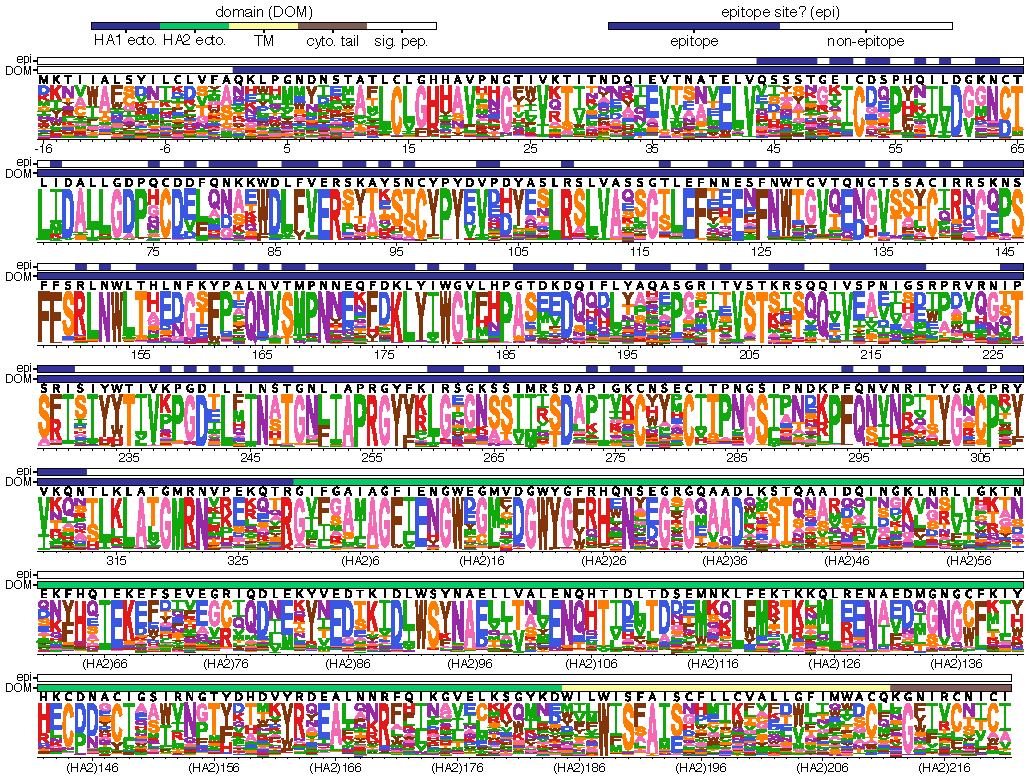
\includegraphics[width=17cm]{figs/prefslogoplot/rescaled-avgprefs_prefs.pdf}
\caption{\label{fig:logoplot}
{\bf The site-specific amino-acid preferences of the Perth/2009 HA measured in our experiments.}
The height of each letter is the preference for that amino acid, after taking the average over experimental replicates and re-scaling~\cite{hilton2017phydms} by the stringency parameter in Table~\ref{tab:phydms}.
The sites are in H3 numbering.
The top overlay bar indicates whether or not a site is in the set of epitope residues delineated in \cite{wolf2006long}.
The bottom overlay bar indicates the HA domain (sig. pep. = signal peptide, HA1 ecto. = HA1 ectodomain, HA2 ecto. = HA2 ectodomain, TM = transmembrane domain, cyto. tail. = cytoplasmic tail).
The letters directly above each logo stack indicate the wildtype amino acid at that site.
}
\end{figure*}

\subsection*{There is less difference in mutational tolerance between the HA head and stalk domains for H3 than for H1}
Our experiments measure which amino acids are tolerated at each HA site under selection for protein function.
We can therefore use our experimentally measured amino-acid preferences to calculate the inherent mutational tolerance of each site, which we quantify as the Shannon entropy of the re-scaled preferences.
In prior mutational studies of the WSN/1933 H1 HA, the stalk domain was found to be substantially less mutationally tolerant than the globular head~\cite{thyagarajan2014inherent,wu2014high,doud2016accurate}.

We performed a similar analysis using the current data for the Perth/2009 H3 HA.
Surprisingly, there was much less contrast in mutational tolerance between the stalk and head domains for the H3 HA than for the H1 (Figure~\ref{fig:mut_tolerance}).
For instance, in the H3 HA, the short helix A in the stalk is very mutationally tolerant.
Interestingly, more studies have reported selecting escape mutants from broadly neutralizing anti-stalk antibodies in H3~\cite{ekiert2011highly, friesen2014common, chai2016two, yamayoshi2017human} than in H1~\cite{okuno1993common,doud2017quantifying} HAs.

We also see high mutational tolerance in many of the known antigenic regions of H3 HA~\cite{wiley1981structural}.
For instance, in recent H3N2 strains, antigenic region B is immunodominant, and most recent major antigenic drift mutations have occurred in this region~\cite{chambers2015identification,koel2013substitutions,popova2012immunodominance}.
We find that the most distal portion of the globular head near the 190-helix, which is part of antigenic region B, is highly tolerant of mutations (Figure~\ref{fig:mut_tolerance}).
Antigenic region C is also notably mutationally tolerant.

Many residues inside HA's receptor binding pocket are known to be highly functionally constrained~\cite{wilson1981structure,martin1998studies}, and our data indicates that these sites are relatively mutationally intolerant in both H3 and H1 HAs.
In contrast, the residues surrounding the receptor binding pocket are fairly mutationally tolerant, which may contribute to the rapidity of influenza's antigenic evolution, since mutations at these sites can have large effects on antigenicity~\cite{wiley1981structural,koel2013substitutions}.

%\begin{SCfigure*}[\sidecaptionrelwidth][t]
\begin{figure}
\centering
%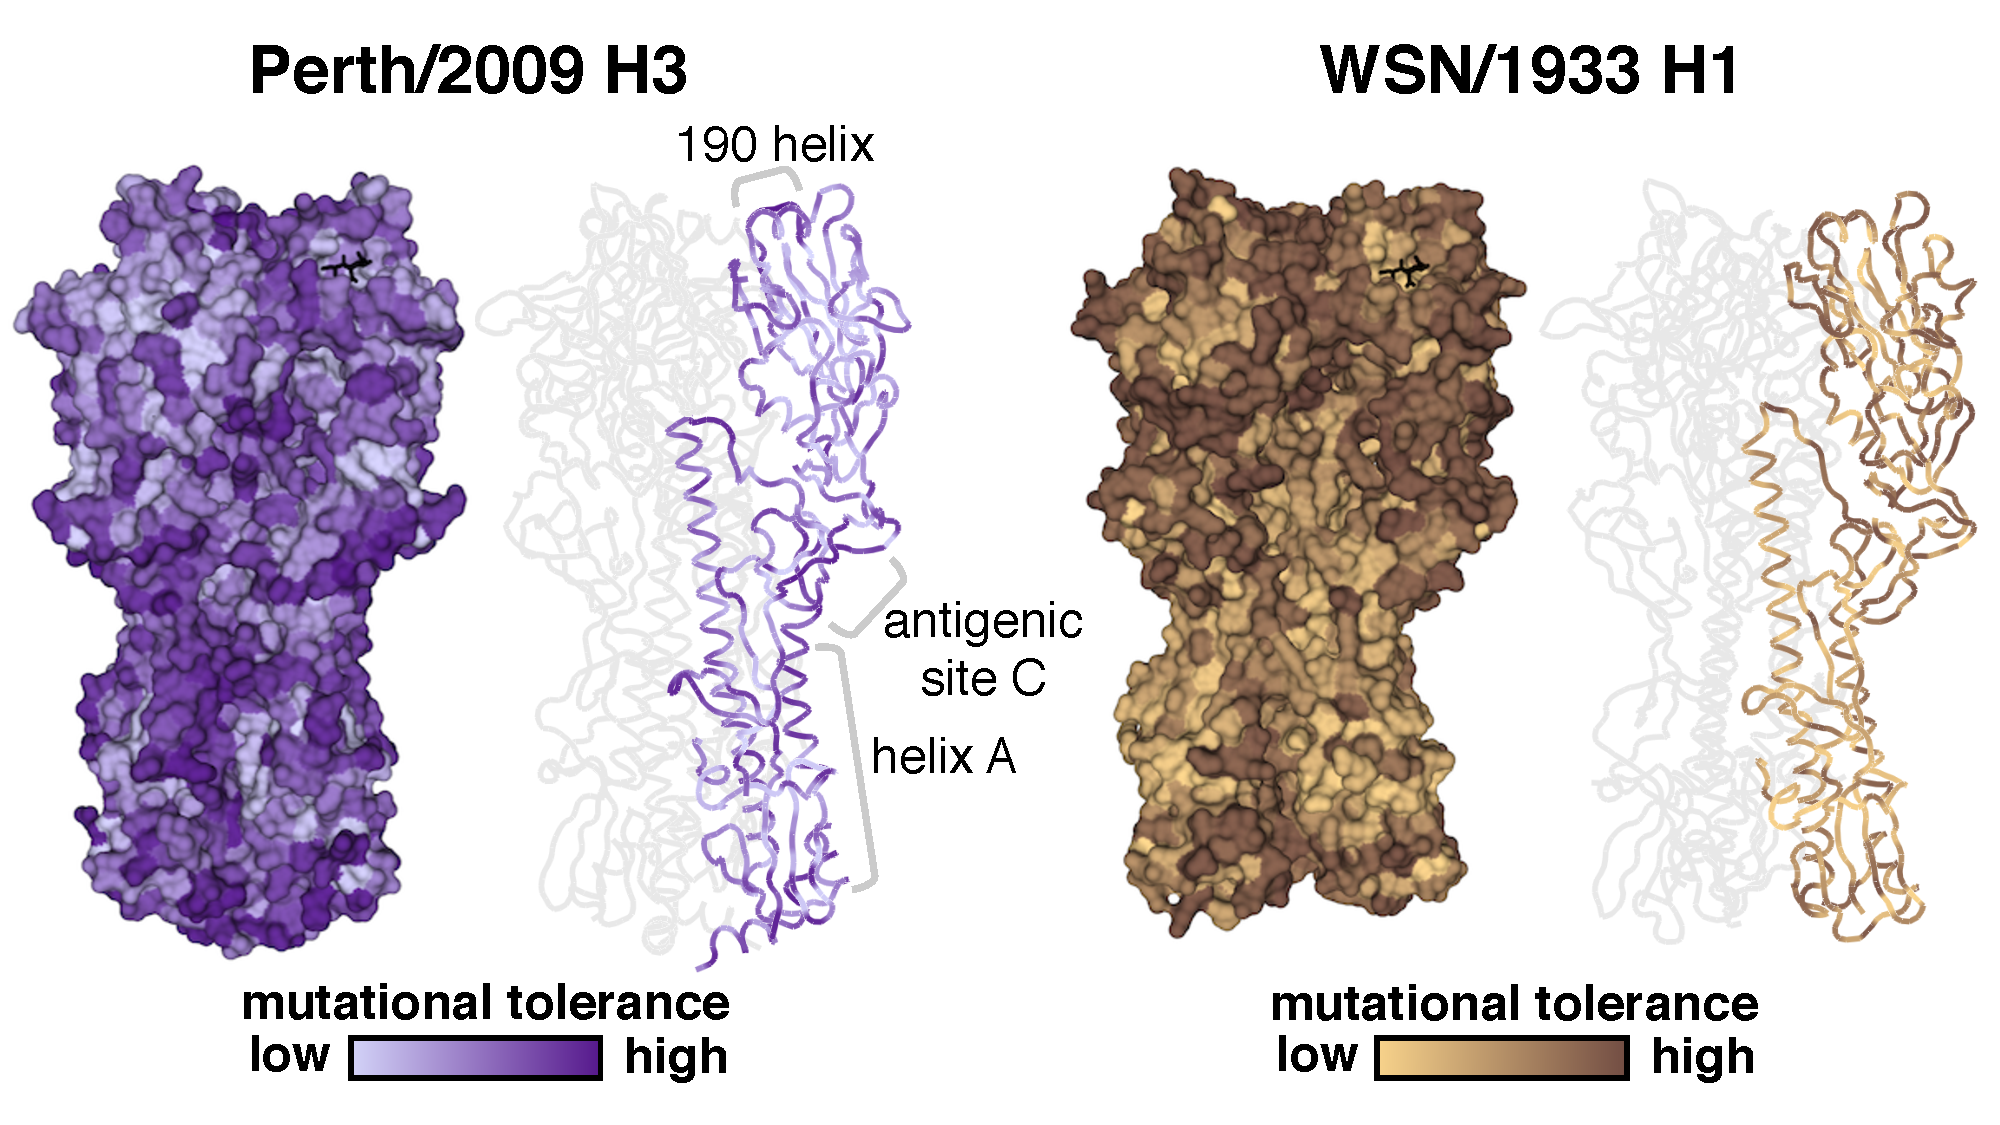
\includegraphics[width=11.4cm]{figs/mut_tolerance/entropy_heatmap.pdf}
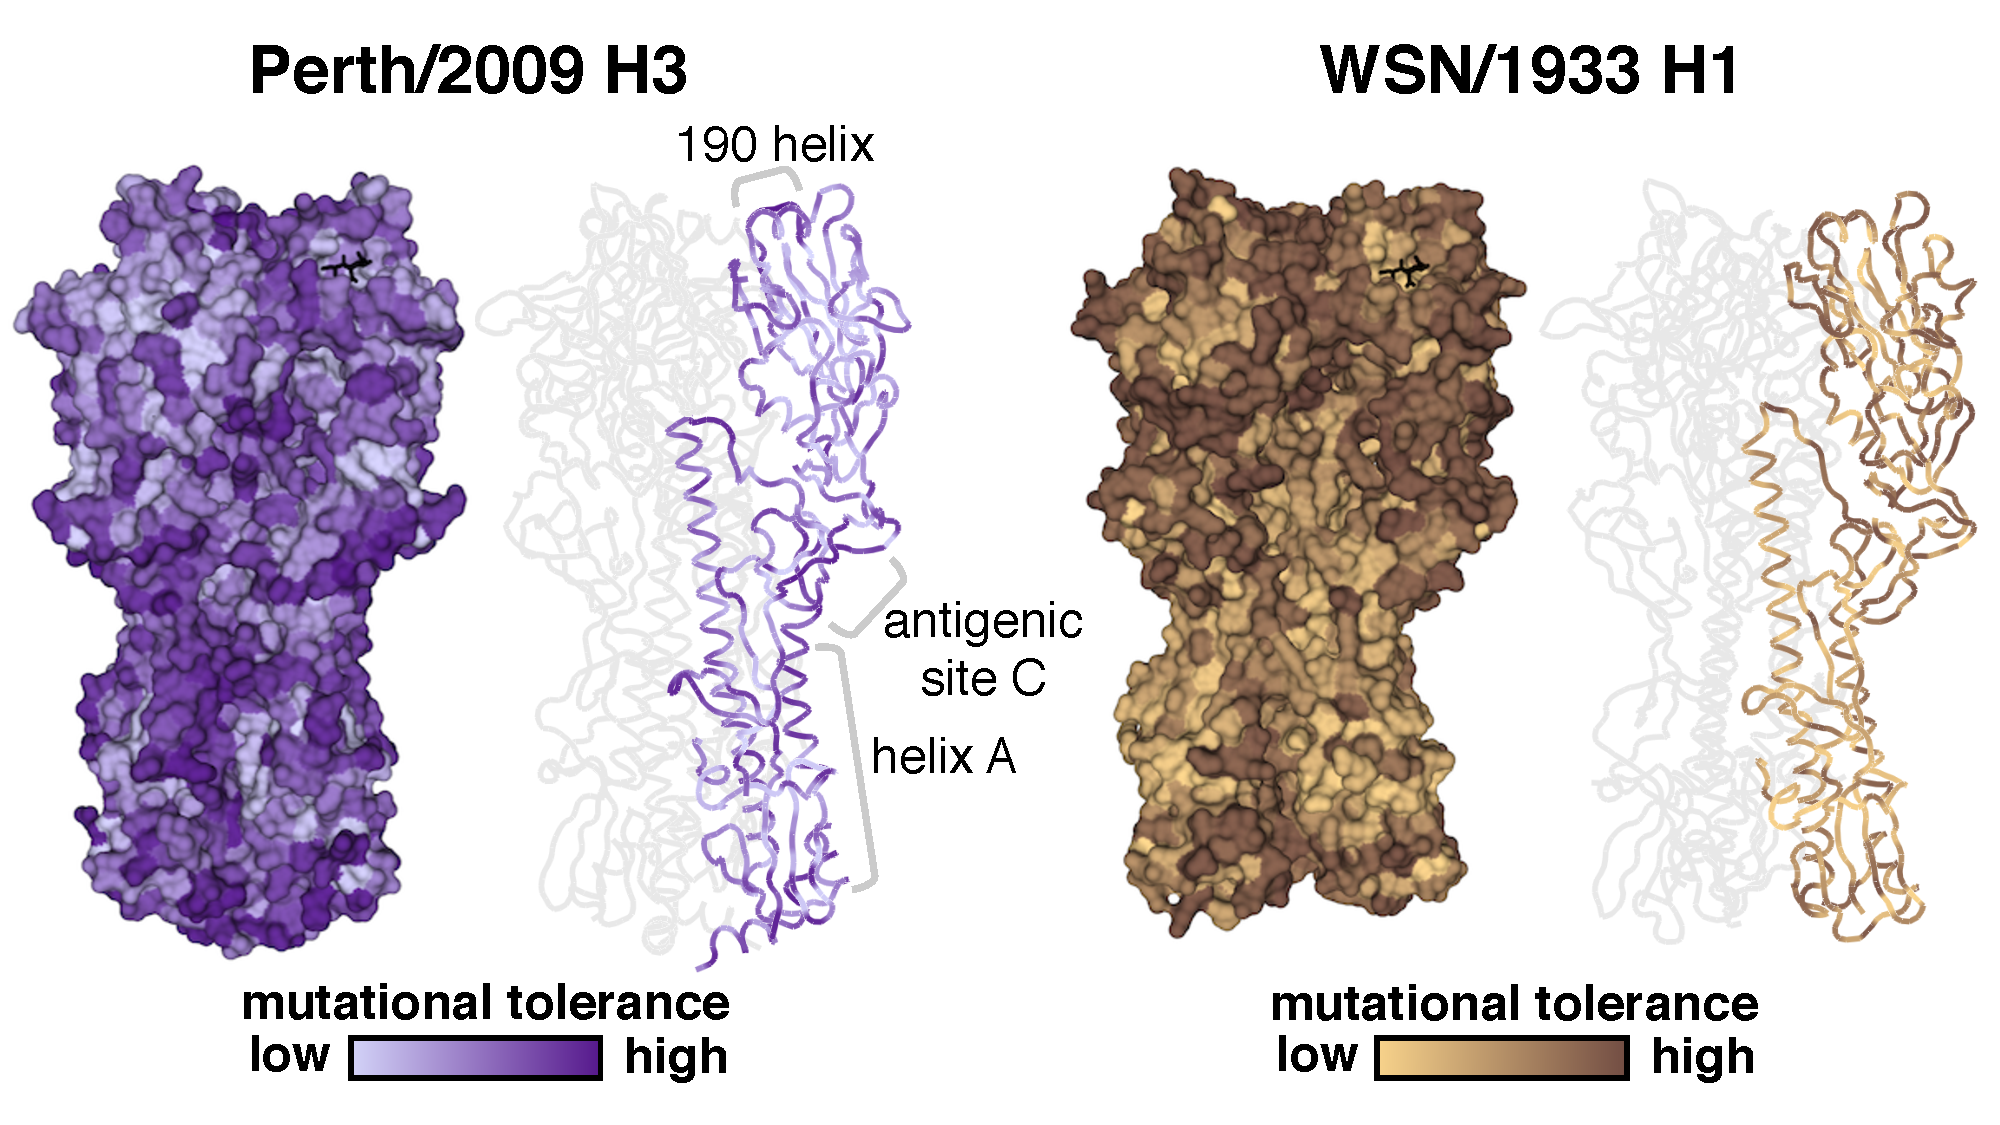
\includegraphics[width=\columnwidth]{figs/mut_tolerance/entropy_heatmap.pdf}
\caption{\label{fig:mut_tolerance}
{\bf Mutational tolerance of each site in H3 and H1 HAs.}
Mutational tolerance as measured in the current study is mapped onto the structure of the H3 trimer (PDB 4O5N;~\cite{lee2014receptor}).
Mutational tolerance of the WSN/1933 H1 HA as measured in \cite{doud2016accurate} is mapped onto the structure of the H1 trimer (PDB 1RVX;~\cite{gamblin2004structure}).
Different color scales are used because measurements are comparable among sites within the same HA, but not necessarily across HAs.
Both trimers are shown in approximately the same orientation. 
For each HA, the structure at left shows a surface representation of the full trimer, while the structure at right side shows a ribbon representation of just one monomer.
The sialic acid receptor is shown in black sticks.
}
%\end{SCfigure*}
\end{figure}

\subsection*{The experimental measurements can help discriminate between successful and unsuccessful influenza virus lineages}
A major goal in the study of rapidly evolving viruses such as influenza is to forecast evolutionary trajectories~\cite{lassig2017predicting,morris2017predictive}.
For instance, forecasting which viral lineages will dominate the upcoming influenza season is an integral part of vaccine-strain selection~\cite{neher2015nextflu,lassig2017predicting,morris2017predictive}. 
Evolutionary forecasts must ultimately distinguish between successful and unsuccessful viral lineages, which in the case of human influenza virus means distinguishing between the trunk and side branches of the phylogenetic tree (Figure~\ref{fig:H3N2_phylogeny}).

To investigate whether our experiments can aid in distinguishing trunk and side branch lineages, we calculated the experimentally measured effects of all mutations in a maximum-likelihood reconstruction of the phylogeny in Figure~\ref{fig:H3N2_phylogeny}.
The mutations that occurred on the trunk of the tree were consistently more beneficial for viral growth according to our experimental measurements (Figure~\ref{fig:trunkvssidebranch}A).
This difference in the effects of mutations between the trunk and side branch lineages was statistically significant when taken across the entire phylogeny (Figure~\ref{fig:trunkvssidebranch}B).
Some influenza sequences are determined using egg- or cell-passaged isolates that contain lab-adaptation mutations~\citep{wu2017structural,mcwhite2016sequence,skowronski2016mutations}.
These mutations mostly occur on the terminal side branches that lead to tip nodes on the phylogenetic tree.
We therefore re-calculated the statistics separating side branches to tip and internal nodes, and again found that the difference between the trunk and both sets of side branches was statistically significant (Figure~\ref{fig:trunkvssidebranch}B).
Therefore, strains with mutations that we experimentally measure to be favorable for viral replication tend to do better in nature than strains with mutations that we measure to be less favorable. 

Our experiments were performed on the Perth/2009 HA, but we are scoring mutations on a phylogenetic tree that extends from 1968 to 2017.
Because the effects of mutations can vary with genetic background~\cite{gong2013stability,natarajan2013epistasis,harms2014historical,starr2016epistasis,starr2017alternative}, it is possible that the effects of mutations that we measured in the Perth/2009 HA might have shifted somewhat in other related HAs.
To explore this question, we scored the complete HA sequence $\mathbf{s}$ of every node in the phylogenetic tree by quantifying its average per-site sequence preference as 
\begin{equation}
F\left(\mathbf{s}\right) = \frac{1}{L}\displaystyle\sum_{r=1}^L \ln \pi_{r, s_r},
\end{equation}
where $\pi_{r, s_r}$ is the preference measured in our experiments (e.g., Figure~\ref{fig:logoplot}) for the amino acid $s_r$ at site $r$ in HA sequence $\mathbf{s}$, and $L$ is the length of the sequence.
Figure~\ref{fig:trunkvssidebranch}C shows that the sequences of trunk nodes tend to have higher preference than those of side branch nodes across the entire timespan, consistent with the finding that trunk mutations are generally more favorable than side branch mutations. 
However, the average per-site sequence preference increases as the nodes approach the Perth/2009 strain.
The Perth/2009 itself has among the highest per-site sequence preference of the entire tree, despite falling on a side branch.
These results suggest that there is some HA background-dependence in the effects of mutations, but that despite this fact our experimental measurements consistently reveal the selective advantage of the trunk over more than a half-century of viral evolution.


\begin{figure}
\centering
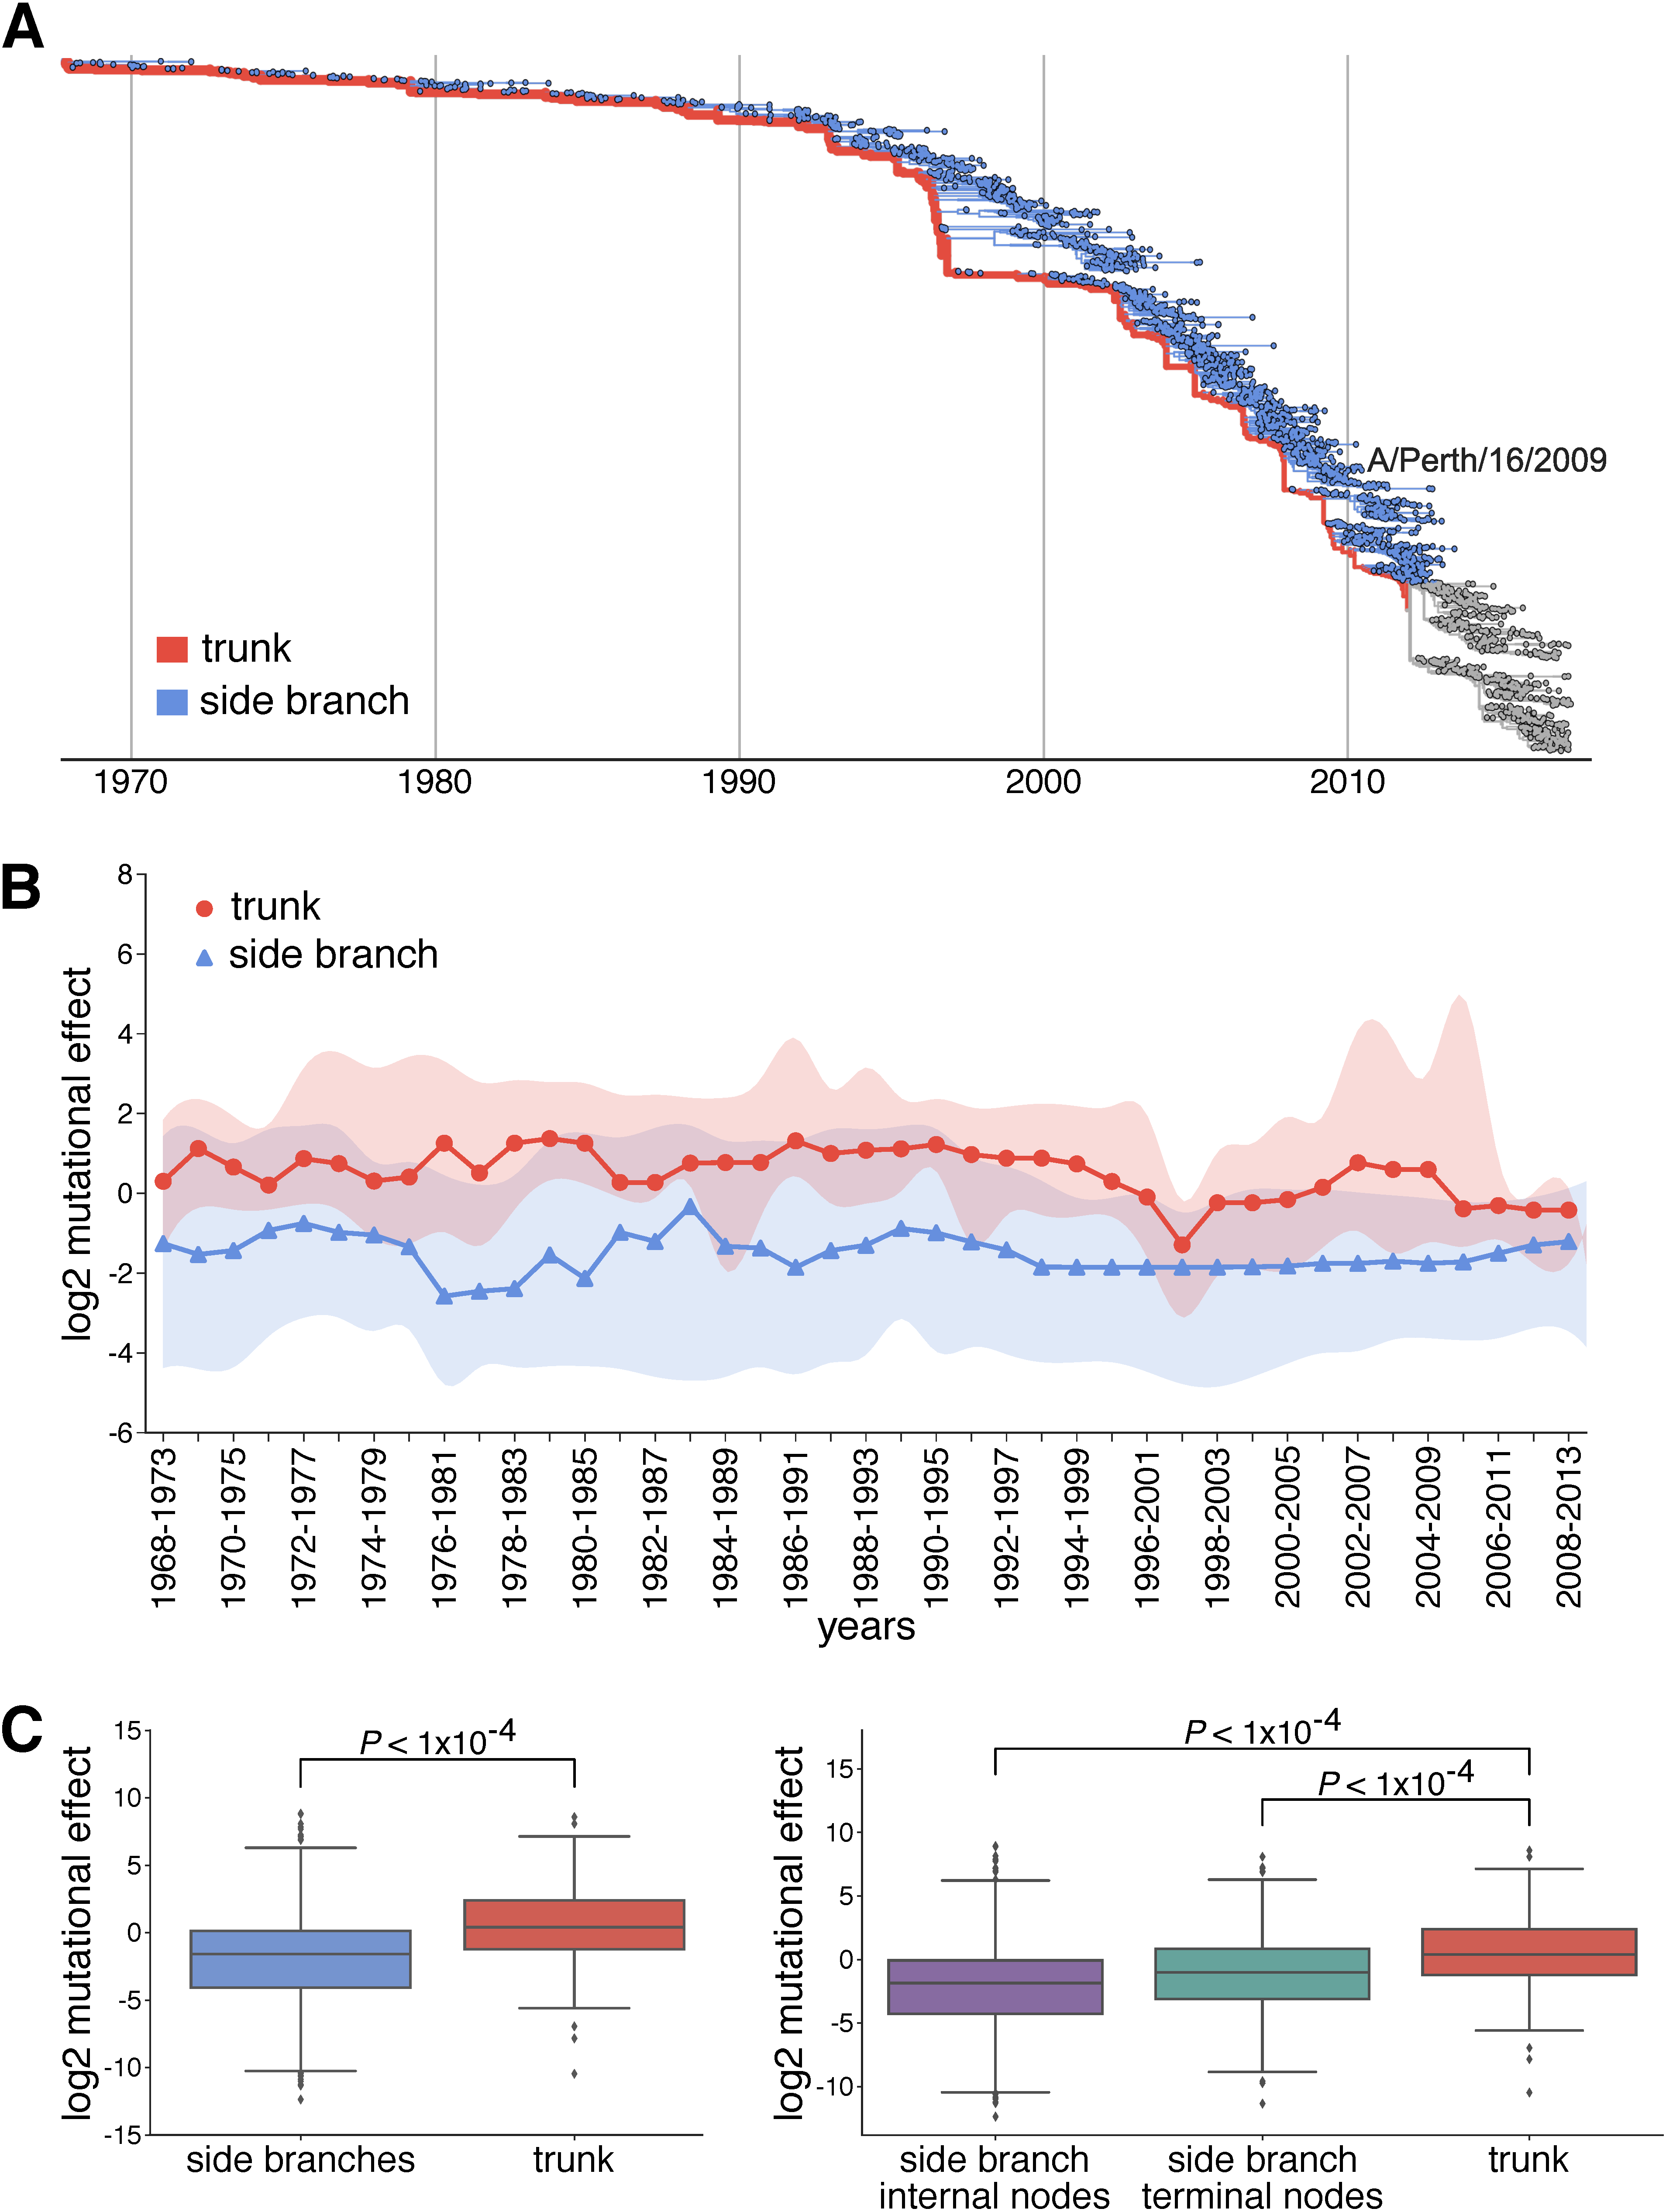
\includegraphics[width=\columnwidth]{figs/trunkvssidebranch/trunkvssidebranch.pdf}
\caption{\label{fig:trunkvssidebranch}
{\bf Mutations on the trunk are more favorable than those on the side branches according to our experimental measurements.}
(A) We used our experiments to calculate the log$_{2}$ mutational effect for all trunk and side branch mutations in five-year windows from 1968 to 2013. 
The central year in each window is denoted on the x-axis.
Median mutational effects in each window are shown as circles for the trunk and triangles for side branches. 
The shaded regions demarcate the interquartile range.
Negative numbers signify mutations towards less preferred amino acids, while positive numbers signify mutations to more preferred mutations.
(B) The log$_{2}$ mutational effect for all side branch and all trunk mutations (left panel), and the same data but separating side branches to terminal and internal nodes.
$P$-values were computed by randomizing the experimental measurements among sites 10,000 times, and determining how often the difference in median mutational effect between the trunk and side branches for the randomized data exceeded the actual value.
(C) The average per-site sequence preference of every node in the phylogenetic tree in Fig.~\ref{fig:H3N2_phylogeny}.
Trunk nodes are in red, side branch nodes in blue, and Perth/2009 is marked with a yellow star.
More preferred sequences have larger values.
}
\end{figure}

\subsection*{Our experiments suggest different patterns of evolution at epitope and non-epitope sites}
HA is under selection both to maintain its essential function in viral growth and to escape pre-existing immunity.
Most immune selection is focused on a subset of so-called ``epitope sites'' that are targets of the immunodominant antibody response.
Although both epitope and non-epitope sites evolve rapidly, immune selection drives a higher rate of evolution at epitope sites\comment{Maybe add some references to this point?}.
There are various classifications of HA epitope sites; here we will use the classification of Wolf \textit{et al}~\cite{wolf2006long}, which defines 129 epitope sites among the 567 residues in HA.
In the timeframe from 1968 to 2012, the trunk of the tree in Figure~\ref{fig:H3N2_phylogeny} fixed 0.84 epitope mutations per site, but only 0.07 non-epitope mutations per site.
Since our experiments only measure how mutations affect viral growth, they might be expected to describe the evolution of epitope and non-epitope sites differently.

Mutations that occur on the trunk are scored as significantly more favorable in our experiments than side-branch mutations at both epitope and non-epitope sites (Figure~\ref{fig:sequence_preference}A).
Therefore, our experiments can distinguish evolutionarily favorable mutations both at sites that are predominantly under functional constraint and at sites that are also under immune pressure.
The fact that our experiments can discriminate between the trunk and side branches at epitope sites despite only assaying for viral growth underscores the fact that most epitope sites are still important for HA function~\cite{nakajima2003restriction,das2013defining,koel2013substitutions}. 

But interestingly, there are clear differences in how the average per-site sequence preference changes over time at the epitope and non-epitope sites (Figure~\ref{fig:sequence_preference}B).
The per-site sequence preference at epitope sites increases over time (Figure~\ref{fig:sequence_preference}B and Figure~\ref{suppfig:seqpref_zoomed}), whereas at non-epitope sites it remains relatively constant.
In addition, the per-site sequence preference is consistently higher at non-epitope than epitope sites, perhaps consistent with the fact that strong immune selection can lead to the fixation of less functionally favorable mutations at epitope sites.
The fact that the epitope sites exhibit more of an increase in sequence preference over time may be due to the fact that they fix more mutations.
It is known that as mutations accumulate at protein sites, they can lead to epistatic shifts in the effects of mutations~\cite{gong2013stability,natarajan2013epistasis,harms2014historical,starr2016epistasis,starr2017alternative,haddox2017mapping}.
Such epistasis has been experimentally demonstrated for HA~\cite{das2013defining,myers2013compensatory}, including at some specific epitope sites in H3 HA~\cite{wu2017diversity}.
It is also known that positive selection for immune escape can increase the amount of epistasis among substitutions by favoring the fixation of combinations of individually deleterious immune-escape mutations and counterbalancing secondary mutations~\cite{gong2014epistatically}.
We hypothesize that immune selection increases the accumulation of epistatic interactions involving substitutions at epitope sites.
Over time, these epistatic interactions could manifest as shifts in the effects of mutations, leading to an apparent increase in per-site sequence preference over time when mutational effects are measured in the Perth/2009 HA.

\begin{figure}
\centering
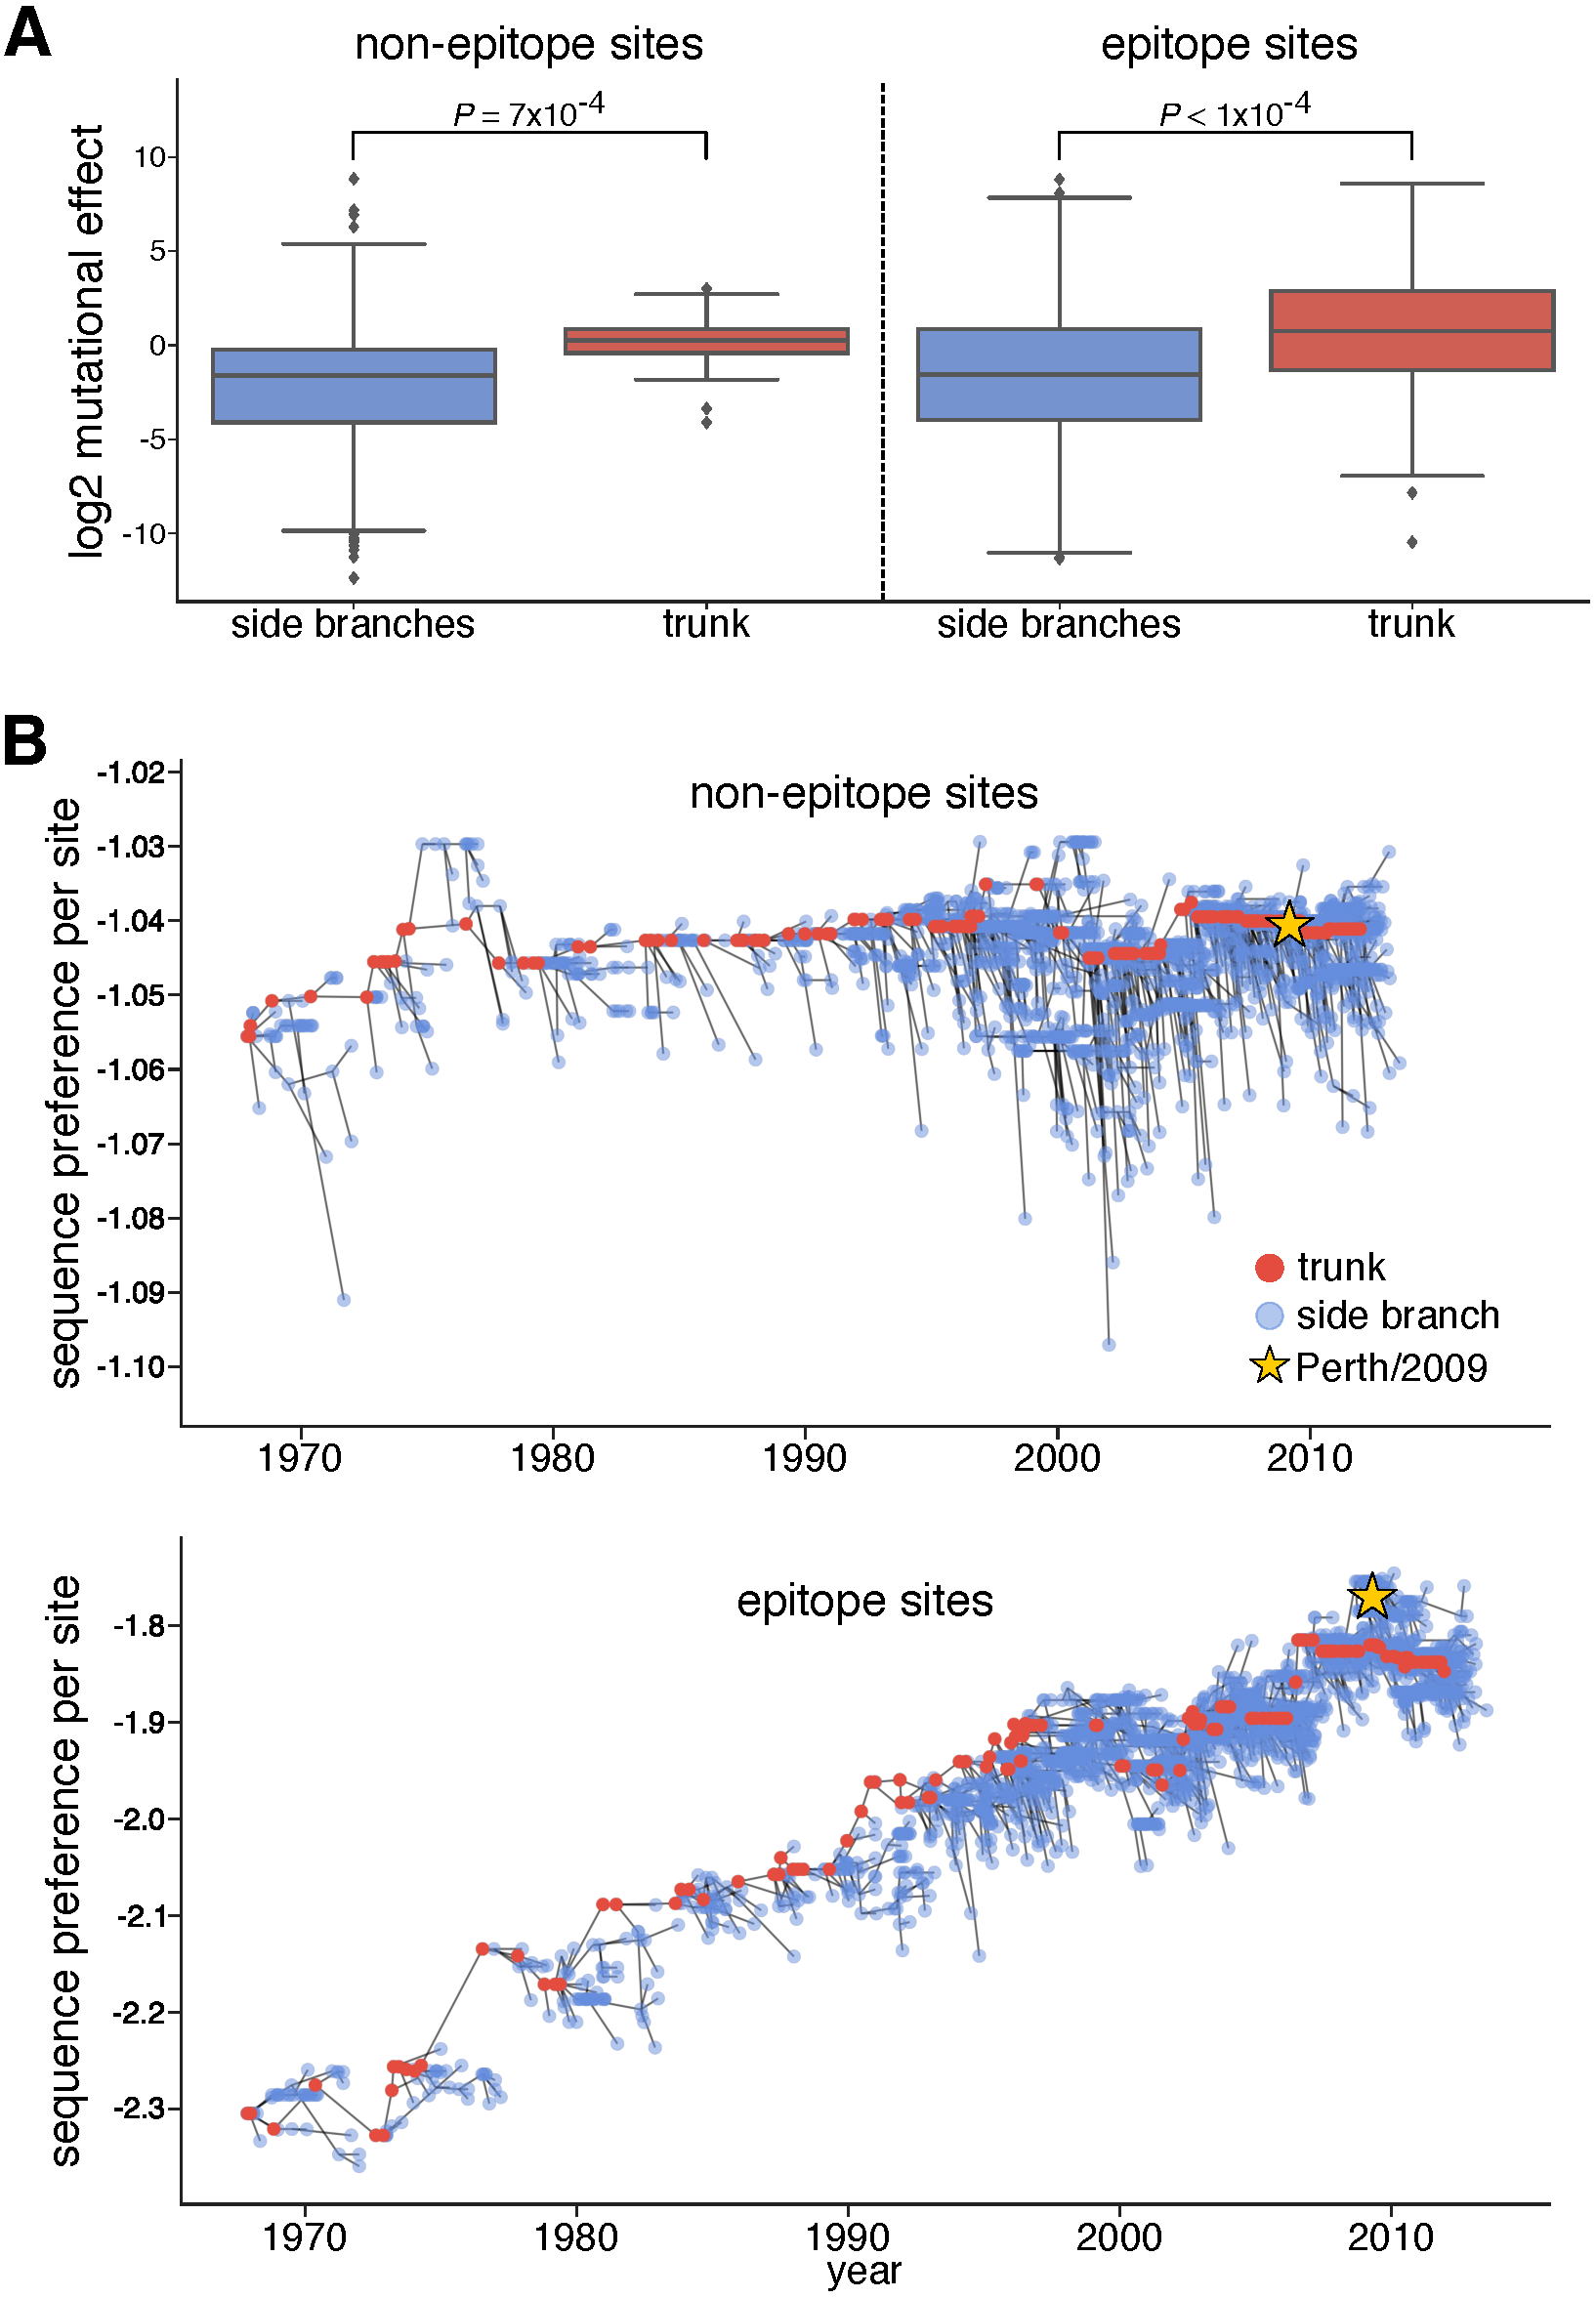
\includegraphics[width=\columnwidth]{figs/sequence_preference/sequence_preference.pdf}
\caption{\label{fig:sequence_preference}
{\bf Effects of mutations at epitope and non-epitope sites during HA evolution.}
We partitioned HA into epitope and non-epitope sites~\cite{wolf2006long}.
(A) The log$_{2}$ mutational effects for side branch and trunk mutations at non-epitope (left) and epitope (right) sites.
$P$-values were computed as in Figure~\ref{fig:trunkvssidebranch} but only performing the randomizations over the appropriate set of sites (non-epitope or epitope).
(B) 
The average per-site sequence preference for all nodes in the phylogenetic tree, calculated separately for each set of sites.
The sequence preferences for epitope and non-epitope sites on separate y-axes is shown in Figure~\ref{suppfig:seqpref_zoomed}.
}
\end{figure}


\subsection*{There are large differences between H3 and H1 HAs in the amino-acid preferences of many sites}
The results above show that measurements of mutational effects in the Perth/2009 HA are informative about the evolutionary fate of other human H3N2 HAs.
How broadly can experimental measurements be generalized across HAs?
To address this question, we repeated the trunk versus side-branch analyses using amino-acid preferences from our prior deep mutational scanning of the WSN/1933 H1 HA, which is highly diverged from the Perth/2009 H3 HA.
Figure~\ref{fig:WSN_trunkvssidebranch} shows that the H1 measurements are not informative for distinguishing the trunk and side branches of an H3 phylogeny.
This fact indicates that the utility of an experiment for discriminating successful and unsuccessful strains degrades over sufficiently long evolutionary distances. 

\begin{figure}
\centering
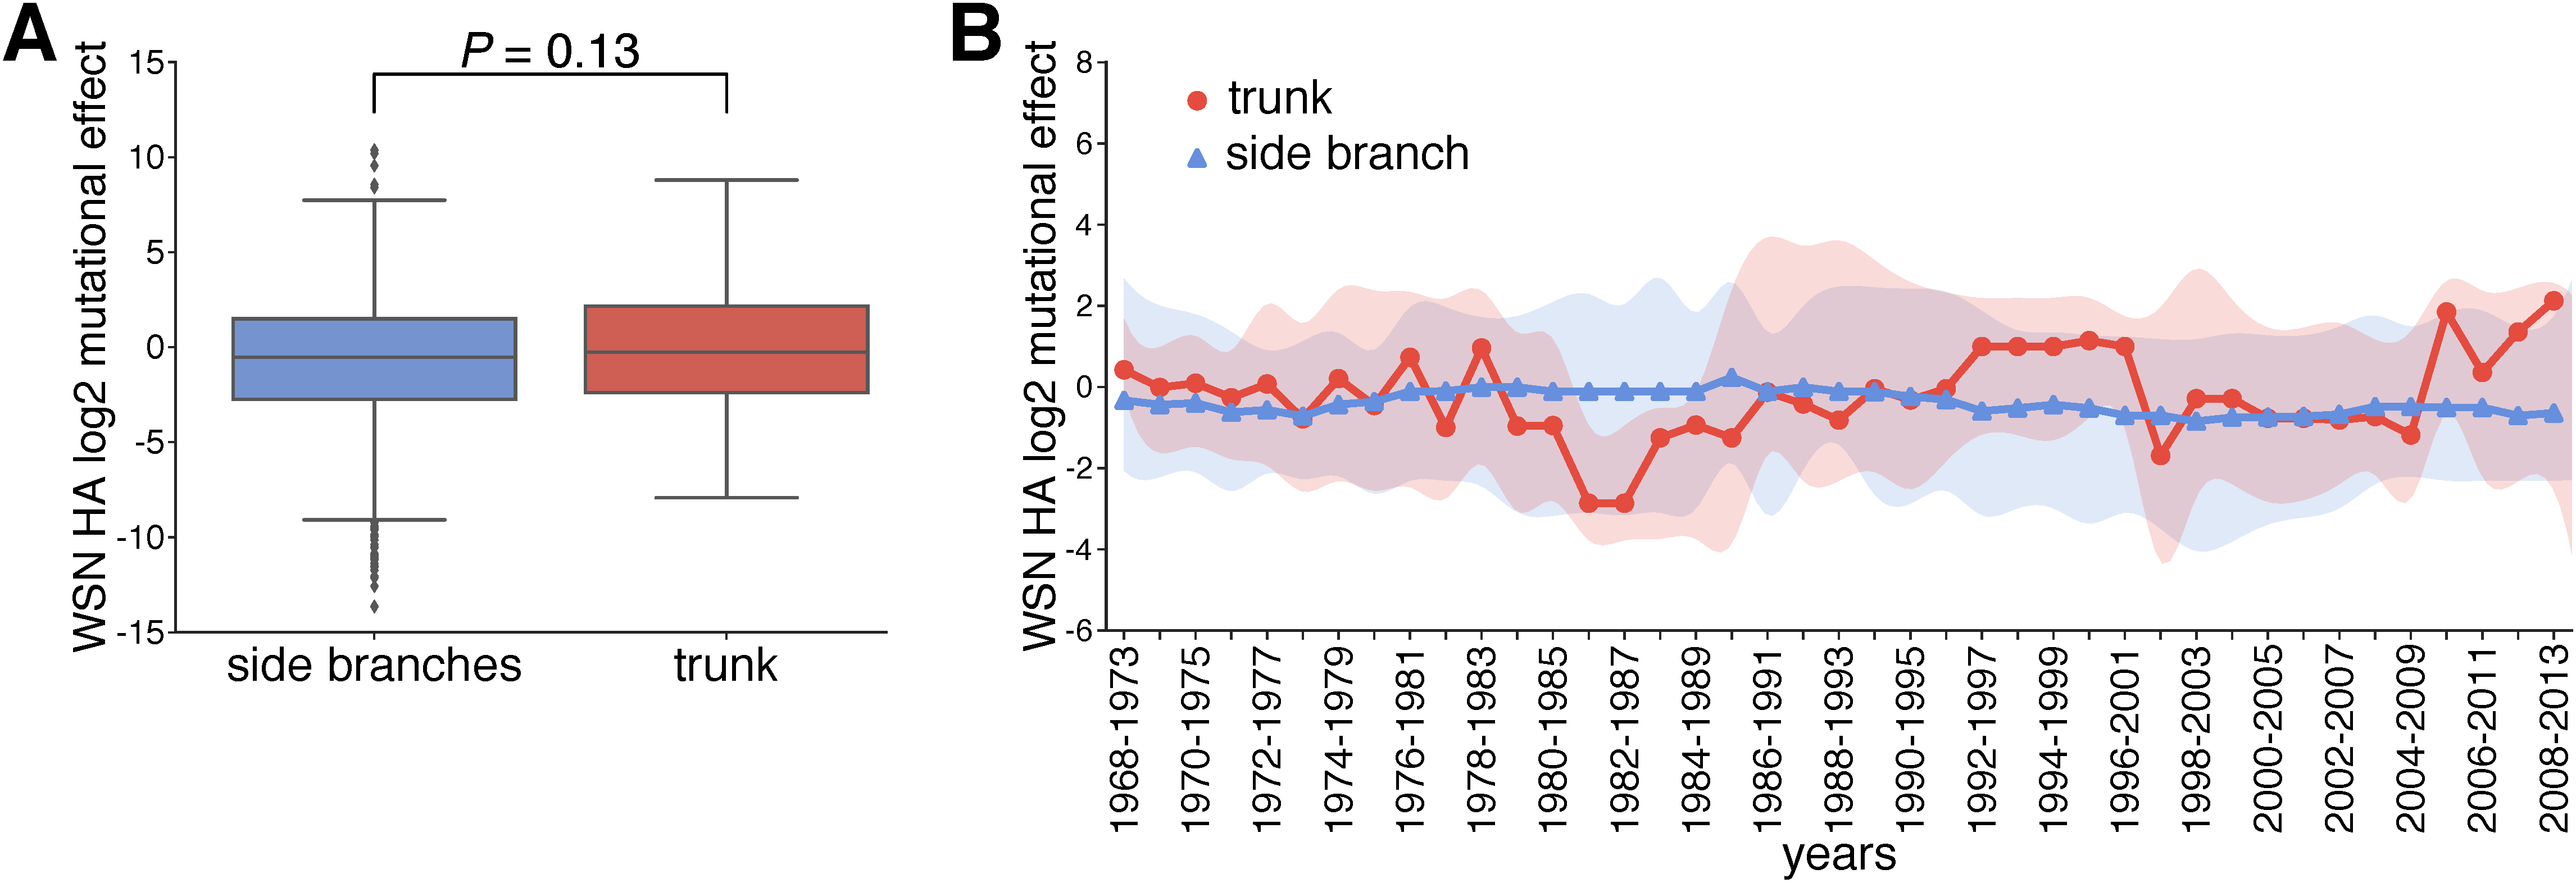
\includegraphics[width=\columnwidth]{figs/WSN_trunkvssidebranch/WSN_trunkvssidebranch.pdf}
\caption{\label{fig:WSN_trunkvssidebranch}
{\bf Experimental measurements on an H1 HA do \emph{not} provide evolutionarily relevant information for H3 HAs.}
(A), (B) This figure is analogous to that in Figure~\ref{fig:trunkvssidebranch} except that it scores the H3 sequences using experimental measurements made on the lab-adapted WSN/1933 HA~\cite{doud2016accurate}.
}
\end{figure}

An obvious hypothesis for why the H1 deep mutational scanning is not informative about the evolutionary fate of H3 strains is that the effect of the same mutation will often be very different between these two HA subtypes.
To determine if this is the case, we can examine how much the amino-acid preferences of homologous sites have shifted between H3 and H1 HAs.
Prior experiments have found only modest shifts in amino-acid preferences between two variants of influenza nucleoprotein with 94\% amino-acid identity~\cite{doud2015site} and variants of HIV envelope (Env) with 86\% amino-acid identity~\cite{haddox2017mapping}.
However, the H1 and H3 HAs are far more diverged, with only 42\% amino-acid identity (Figure~\ref{fig:distance_distribution}A).
One simple way to investigate the extent of shifts in amino-acid preferences is simply to correlate measurements from independent deep mutational scanning replicates on H1 and H3 HAs.
Figure~\ref{fig:distance_distribution}B clearly reveals that replicate measurements on the same HA variant are more correlated than those on different HA variants.

To more rigorously quantify shifts in amino-acid preferences after correcting for experimental noise, we used the statistical approach described in~\cite{doud2015site,haddox2017mapping}.
Figure~\ref{fig:distance_distribution}C shows the distribution of shifts in amino-acid preferences between H3 and H1 HAs after correcting for experimental noise.
Although some sites have small shifts near zero, many sites have large shifts in preference.
These shifts between H3 and H1 are much larger than expected from the null distribution that would be observed purely from experimental noise.
They are also much larger than the shifts previously observed between two HIV Envs with 86\% amino-acid identity~\cite{haddox2017mapping}.
However, the shifts are still generally smaller than those observed when comparing HA to the non-homologous HIV Env protein. 
These observations show that there are very substantial shifts in mutational effects between highly diverged HA homologs, although the effects of mutations still remain more similar than for non-homologous proteins.

\begin{SCfigure*}[\sidecaptionrelwidth][t]
\centering
\includegraphics[width=12cm]{figs/distance_distribution/distance_distribution.pdf}
\caption{\label{fig:distance_distribution}
{\bf There are substantial differences in the effects of mutations between H1 and H3 HAs.}
(A) Phylogenetic tree of HA subtypes, with the WSN/1933 H1 and Perth/2009 H3 HAs labeled. 
These HAs have 42\% amino-acid identity.
(B) All pairwise correlations of the amino-acid preferences measured in the three individual deep mutational scanning replicates in the current study  and the three replicates in prior deep mutational scanning of an H1 HA~\cite{doud2016accurate}.
Comparisons between H3 replicates are in purple, those between H1 replicates are in brown, and those across H1 and H3 replicates are in gray. 
$R$ indicates the Pearson correlation coefficient.
(C) We calculated the shift in amino-acid preferences at each site between H3 and H1 HAs using the method in \cite{haddox2017mapping}, and plotted the distribution of shifts for all sites.
The shifts between H3 and H1 (yellow) are much larger than the null distribution (blue) expected if all differences are due to experimental noise.
The shifts are also much larger than those previously observed between two variants of HIV envelope protein (Env) that share 86\% amino-acid identity (pink).
However, the shifts between H3 and H1 are still less than the differences between either HA and HIV Env (green).
}
\end{SCfigure*}

\subsection*{Properties associated with the shifts in amino-acid preferences between H3 and H1 HAs}
What features distinguish the sites that have shifted versus conserved amino-acid preferences between H3 and H1 HAs?
The sites of large shifts are spread across HA, and do not obviously localize to one specific region of the protein's structure (Figure~\ref{fig:RMSD_heatmap}A).
However, at the domain level, sites in HA's stalk tend to have smaller shifts than sites in HA's globular head (Figure~\ref{fig:RMSD_heatmap}B). 
The HA stalk domain is also more conserved at the amino-acid level across HA subtypes~\cite{nobusawa1991comparison,hai2012influenza,mallajosyula2014influenza}, suggesting that conservation of amino-acid sequence tends to be correlated with conservation of amino-acid preferences.
Consistent with this idea, sites that are absolutely conserved across all 18 HA subtypes are significantly less shifted than sites that are variable across HA subtypes (Figure~\ref{fig:RMSD_heatmap}B).
Presumably these sites are under consistent functional constraint across all HAs.

Despite their high sequence divergence, H1 and H3 adopt very similar protein folds~\cite{ha2002h5,russell2004h1}.
However, there are differences in the rotation and upward translation of the globular head subdomains relative to the central stalk domain among different HA subtypes~\cite{ha2002h5,russell2004h1}.
Previous work has defined clades of structurally related HA subtypes~\cite{ha2002h5,russell2004h1}. 
One such clade includes H1, H2, H5, and H6, whereas another clade includes H3, H4, and H14 HAs (Figure~\ref{fig:distance_distribution}).
Sites that are conserved at different amino-acid identities in these two clades tend to have exceptionally large shifts in amino acid preferences (Figure~\ref{fig:RMSD_heatmap}B).
The clade containing H1 has an upward shift of the globular head relative to the clade containing H3.
This structural shift has been attributed largely to the interaction between sites 107 and 75(HA2)~\cite{ha2002h5,russell2004h1}.
Specifically, the clade containing H1 has a taller turn in the interhelical loop connecting helix A and helix B in the stalk domain, and this tall turn is stabilized by a hydrogen bond between Glu-107 and Lys-75(HA2) (Figure~\ref{fig:RMSD_heatmap}C).
In deep mutational scanning of the WSN/1933 H1 HA, site 107 has a high preference for Glu and 75(HA2) strongly prefers positively charged Lys and Arg.
In contrast, the interhelical loop in H3 HA makes a sharper and shorter turn which is facilitated by a Gly at 75(HA2).
In the deep mutational scanning of the Perth/2009 H3 HA, site 75(HA2) prefers Gly and to a lesser extent Val, while site 107 is fairly tolerant of mutations suggesting that the amino-acid identity at this site plays a smaller role in determining the conformation of the interhelical loop.
Therefore, some of the shifts in HA amino-acid preferences can be directly rationalized in terms of changes in HA structure.

\begin{SCfigure*}[\sidecaptionrelwidth][t]
\centering
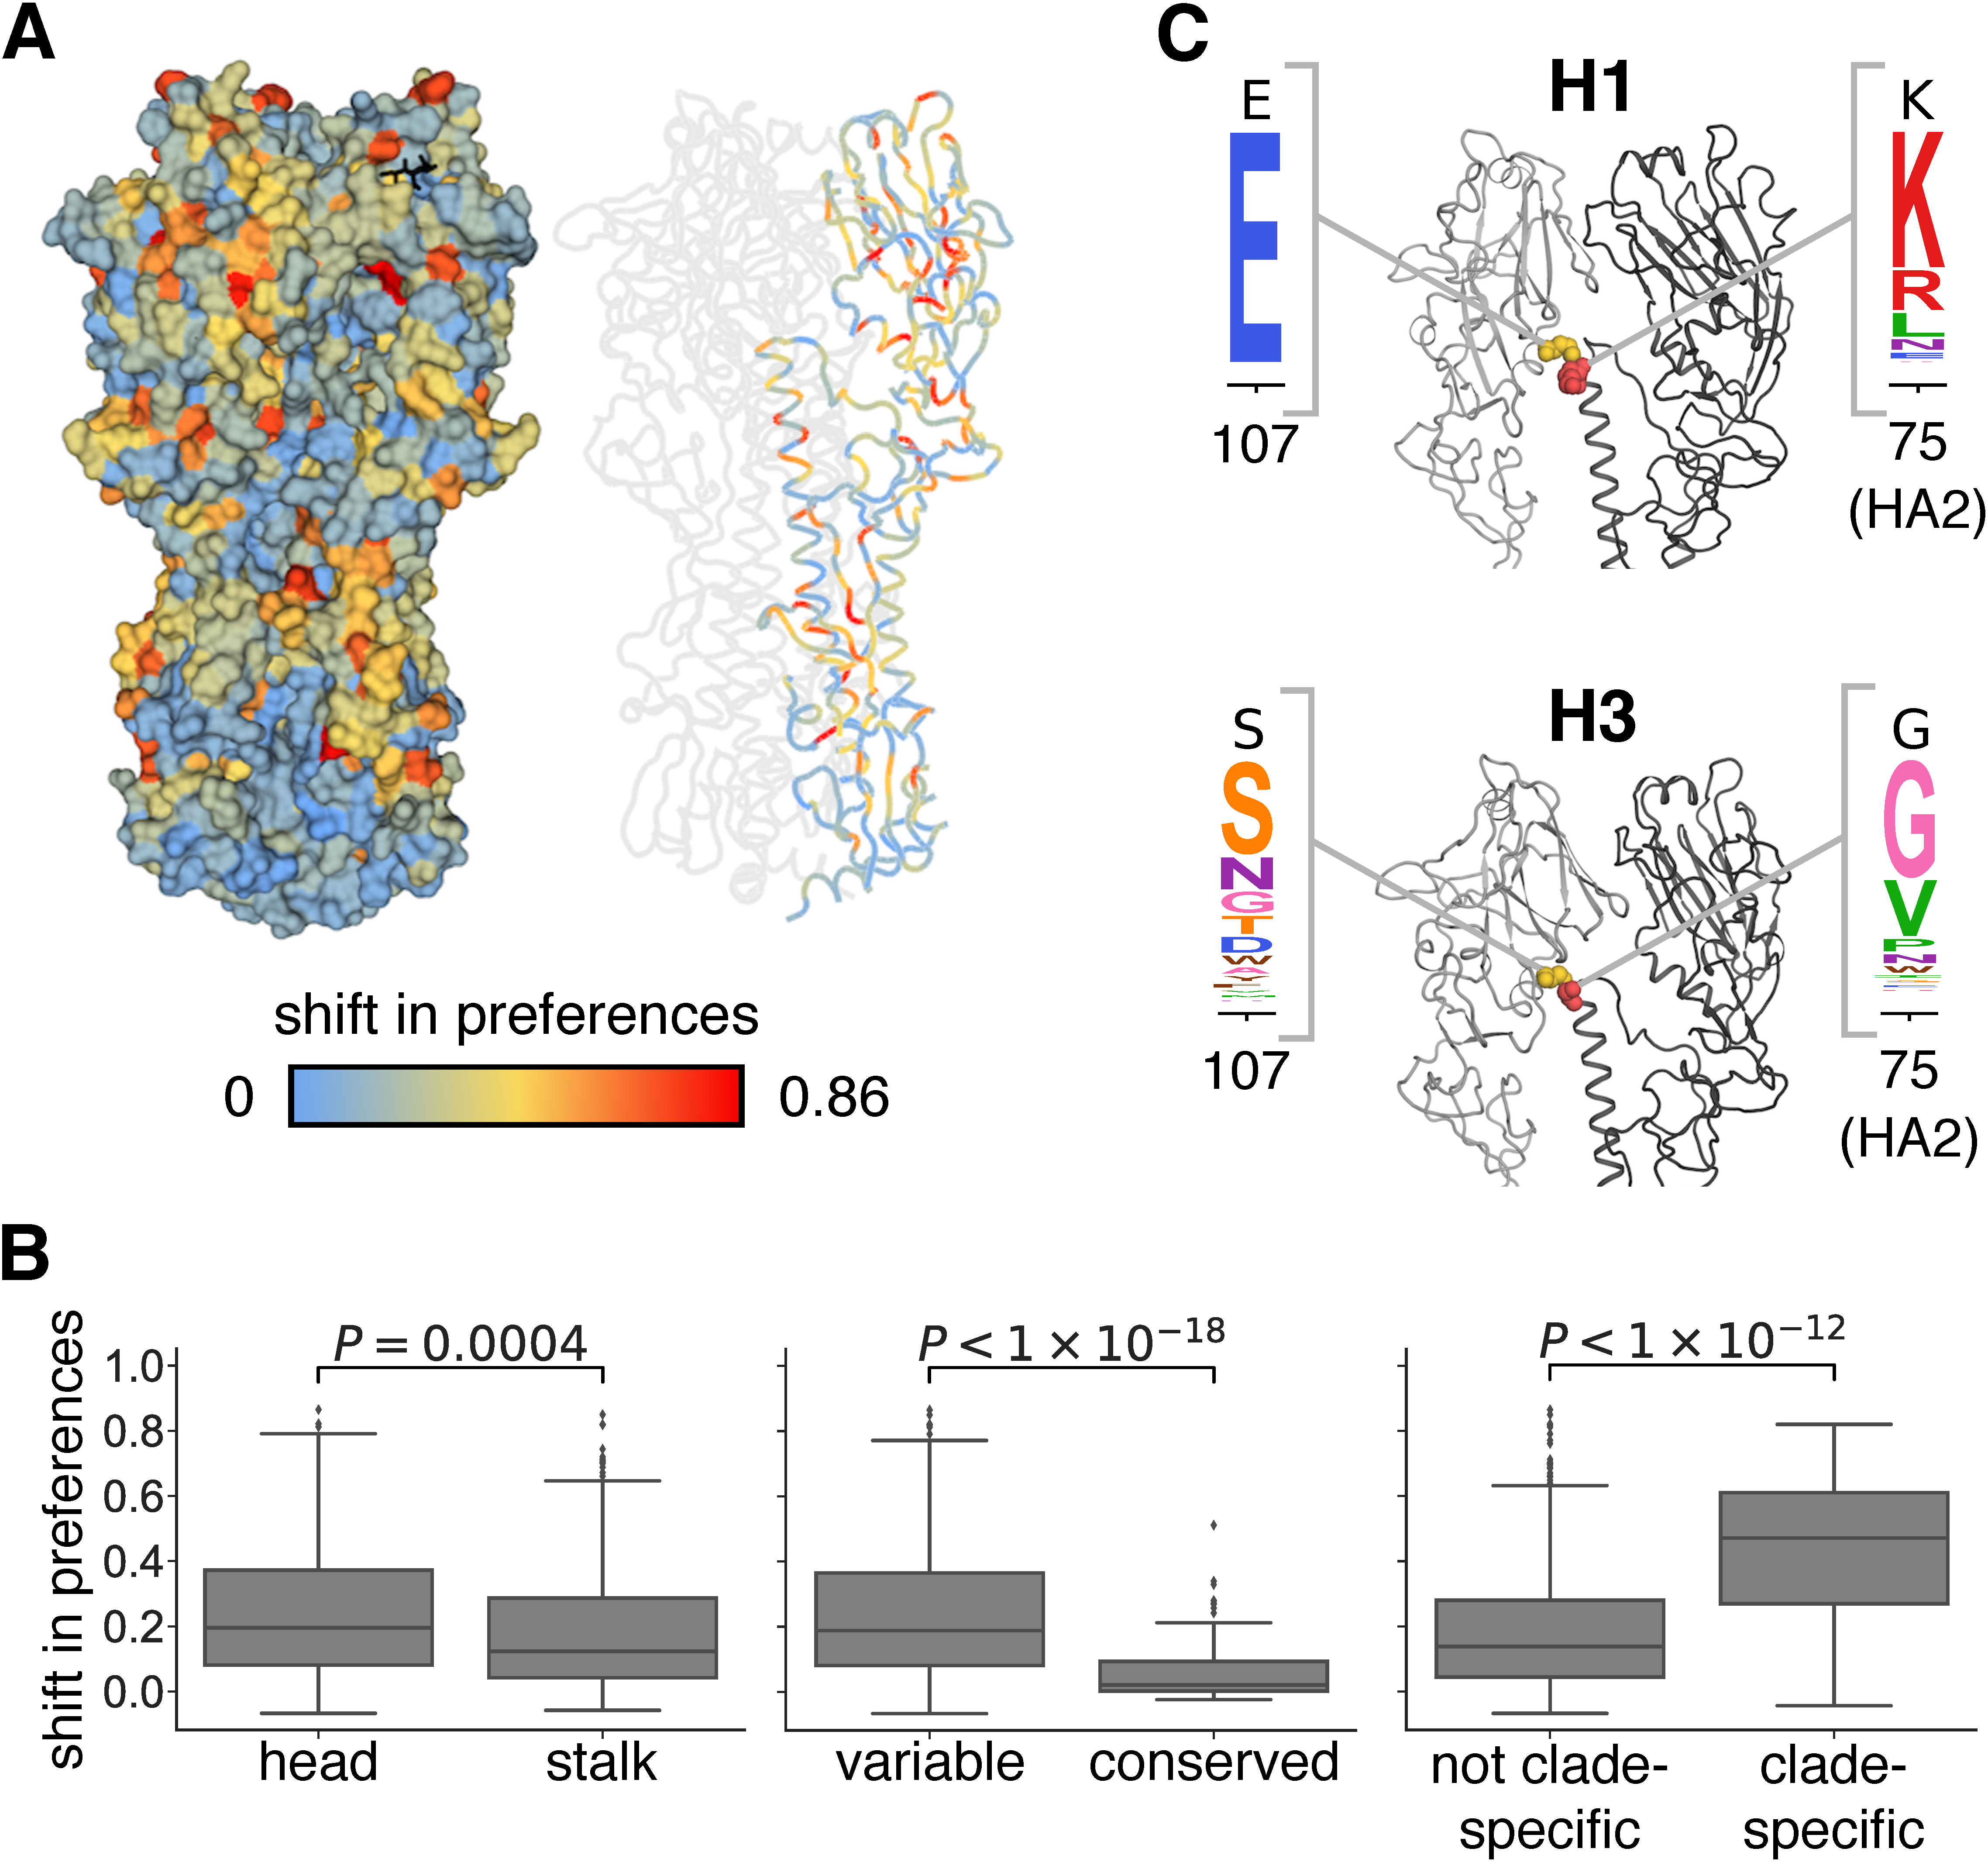
\includegraphics[width=11.4cm]{figs/RMSD_heatmap/RMSD_heatmap.pdf}
\caption{\label{fig:RMSD_heatmap}
{\bf Sites with strongly shifted amino-acid preferences between H3 and H1 HAs.}
(A) The shift in amino-acid preferences between the H3 and H1 HA at each site as calculated in Figure~\ref{fig:distance_distribution}C is mapped onto the structure of the H3 HA. 
(B) Amino-acid preferences of sites in the stalk domain are less shifted than those in the head domain.
Sites absolutely conserved in all 18 HA subtypes are less shifted than other sites.
Sites with one amino-acid identity in the clade containing H1, H2, H5, and H6 and another identity in the clade containing H3, H4, and H14 are more shifted than other sites.
(C) Sites 107 and 75(HA2) help determine the different orientation of the globular head domain in H1 versus H3 HAs.
These sites are shown in spheres on the structure of H1 and H3. 
One monomer is in dark gray, while the HA1 domain of the neighboring monomer is in lighter gray.
The spheres are colored as in panel (A), and the experimentally measured amino-acid preferences in the WSN/1933 H1 and Perth/2009 H3 HAs are shown.
\comment{Could B be a thinner panel at the bottom, and then C be to the right of A, possibly with H1 and H3 vertically oriented? It may be OK to shrink the A panel a bit if that save space in this new layout.}
}
\end{SCfigure*}

\section*{Discussion}
\label{sec:discussion}
We have measured the effect of all possible single amino-acid mutations to Perth/2009 H3 on viral growth in cell culture.

\begin{itemize}
\item{These experimental measurements have utility in revealing differences between successful and unsuccessful lineages over 50 y of human influenza virus evolution.}
\item{We have only measured the effect of mutations to HA on viral growth, but there are certainly other determinants of strain success}
\item{Antigenic characteristics play a large role in determining strain success. We therefore need to know how mutations affect antigenicity.}
\item{non-HA segments are important too}
\end{itemize}

\matmethods{Please describe your materials and methods here. This can be more than one paragraph, and may contain subsections and equations as required. Authors should include a statement in the methods section describing how readers will be able to access the data in the paper.

\subsection*{HA numbering}
Unless otherwise indicated, all sites are in H3 numbering, with the signal peptide in negative numbers, the HA1 subunit in plain numbers, and the HA2 subunit denoted with "(HA2)". The conversion between sequential numbering of the A/Perth/16/2009 HA and H3 numbering was performed using an HA numbering Python script (available at \url{https://github.com/jbloomlab/HA_numbering}).

\subsection*{Creation of MDCK-SIAT1-TMPRSS2 cell line}
The human TMPRSS2 cDNA ORF was ordered from OriGene (NM\_005656), PCR amplified, and cloned into a pHAGE2 lentiviral vector under an EF1$\alpha$-Int promoter and attached to mCherry through an IRES. 
We generated lentiviruses..etc etc transduced MDCK-SIAT1 cells, sorted by fluorescence activated cell sorting
\comment{Need to look at Katie's notebooks for this...}

\subsection*{Generation of HA codon mutant plasmid libraries}
Recombinant A/Perth/16/2009 (HA, NA) $\times$ A/Puerto Rico/8/1934 influenza virus, NIB-64, NR-41803 was ordered from BEI Resources, NIAID, NIH. 
Bulk RNA from the viral sample was extracted using the QIAamp Viral RNA Mini Kit (QIAGEN) according to manufacturer's instructions.
The Perth/2009 HA and NA genes were then reverse transcribed using the SuperScript III First-Strand Synthesis SuperMix Kit (Invitrogen), PCR amplified, and cloned into the pHW2000~\citep{hoffmann2000dna} and pICR2 \comment{cite?} plasmid backbones by In-Fusion.

To generate wildtype Perth/2009 H3N2 virus, we transfected a co-culture of 293T and MDCK-SIAT1-TMPRSS2 cells with reverse genetics plasmids encoding the Perth/2009 HA and NA, WSN/1933 internal genes, and the TMPRSS2 lentiviral vector.
\comment{add more details about reverse genetics?}
The viral supernatant was harvested at 72 hours post-transfection, clarified at 1200 rpm for 5 min, and 0.01 to 1.0 ul of the supernatant was passaged onto $4 \times 10^{5}$ MDCK-SIAT1-TMPRSS2 cells in six-well plates for a total of six serial passages.
After the final passage, RNA was extracted from 140 ul of the viral supernatant using the QIAamp Viral RNA Mini Kit.
The HA and NA genes were reverse transcribed, PCR amplified, and sequenced by Sanger sequencing.
Two mutations, G78D and T212I, arose after serial passaging. 
The Perth/2009 HA carrying these two mutations were cloned into the pHW2000~\citep{hoffmann2000dna} and pICR2 \comment{cite?} plasmid backbones.

The codon-mutant libraries were generated in the Perth/2009 HA-G78D-T212I background using a PCR-based approach described in~\cite{bloom2014experimentally,dingens2017comprehensive} using two rounds of mutagenesis.
The codon mutations were introduced into three independent replicates of the Perth/2009 HA variant.
The mutant variants were then cloned into the pICR2 vector by digestion with BsmBI restriction sites, ligation by T4 DNA ligase, and electroporation and transformation into ElectroMAX DH10B competent cells (Invitrogen; 18290015). 
We pooled over 6 million transformants for each replicate, cultured in liquid LB + ampicillin at 37$^{\circ}$C for 3 h with shaking, and maxiprepped.

\subsection*{Generation and passaging of mutant viruses}
The mutant virus libraries were generated and passaged using the approach described in~\cite{doud2016accurate} with several modifications.
We used the HA-deficient WSN/1933 helper virus generated in~\cite{doud2016accurate}.
Briefly, these helper viruses were generated by transfecting seven WSN/1933 non-HA reverse-genetics plasmids plus a WSN/1933 HA protein expression plasmid into a coculture of 293T and MDCK-SIAT1-EF1$\alpha$-WSN-HA cells engineered to constitutively express the WSN/1933 HA.
The transfection supernatant was then expanded by passaging onto a monolayer of MDCK-SIAT1-EF1$\alpha$-WSN-HA cells, and the viral supernatant was then harvested and aliquots were frozen at -80$^{\circ}$C.

To generate the mutant virus libraries, we transfected $5 \times 10^5$ MDCK-SIAT1-TMPRSS2 cells in suspension with 937.5 ng each of four protein expression plasmids encoding the ribonucleoprotein complex (HDM-Nan95-PA, HDM-Nan95-PB1, HDM-Nan95-PB2, and HDM-Aichi68-NP)~\cite{gong2013stability}, and 1250 ng of one of the three pICR2-mutant-HA libraries (or the wildtype pICR2-Perth2009-HA-G78D-T212I control) using Lipofectamine3000 (ThermoFisher;L3000008).
We allowed the transfected cells to adhere in 6-well plates, then four hours later changed the media to D10 media (DMEM supplemented with 10\% heat-inactivated FBS, 2 mM L-glutamine, 100 U of penicillin/mL, and 100 $\mu$g of streptomycin/mL).
Eighteen hours after transfection, we infected the cells with WSN/1933 HA-deficient helper virus by preparing an inoculum of 500 TCID$_{50}$ per $\mu$L in influenza growth media (Opti-MEM supplemented with 0.01\% heat-inactivated FBS, 0.3\% BSA, 100 U of penicillin/mL, 100 $\mu$g of streptomycin/mL, and 100 $\mu$g of calcium chloride/mL), and aspirating the D10 media from the cells, and adding 2 mL of the helper-virus inoculum to each well.
After three hours, we changed the media to fresh influenza growth media.
Twenty-four hours after helper-virus infection, we harvested the viral supernatants for each replicate, froze aliquots at -80$^{\circ}$C, and titered in MDCK-SIAT1-TMPRSS2 cells.

We passaged over $9 \times 10^5$ TCID$_{50}$ of the transfection supernatants at an MOI of 0.0035 TCID$_{50}$ per cell.
To passage, we plated $4.6 \times 10^6$ MDCK-SIAT1-TMPRSS2 cells per dish in 15-cm dishes in D10 media, and allowed the cells to grow for 24 hours, at which the cells reached a density of $\sim 1.7 \times 10^7$ cells per dish.
We then replaced the media of each dish with 25 mL of an inoculum of 2.5 TCID$_{50}$ of virus per $\mu$L.
We collected viral supernatant for sequencing 48 hours post-infection.

\subsection*{Barcoded subamplicon sequencing}
To extract viral RNA from the three replicate HA virus libraries and the wildtype HA virus, we first ultracentrifuged 24 mL of the supernatant at 22,000 rpm for 1.5 h at 4$^{\circ}$C in a Beckman Coulter SW28 rotor.
We then extracted the RNA using the Qiagen RNeasy Mini Kit by resuspending the viral pellet in 400 $\mu$L of buffer RLT supplemented with $\beta$-mercaptoethanol, pipetting 30 times, transferring the liquid to a microcentrifuge tube, adding 600 $\mu$L 70\% ethanol, and proceeding with the rest of the extraction according to manufacturer's instructions.
The HA gene was then reverse-transcribed with AccuScript Reverse Transcriptase (Agilent 200820) using the primers P09-HA-For (5'-AGCAAAAGCAGGGGATAATTCTATTAATC-3') and P09-HA-Rev (5'-AGTAGAAACAAGGGTGTTTTTAATTACTAATACAC-3').

We generated the HA PCR amplicons for each of the three plasmid libraries, the three virus libraries, one wildtype plasmid, and one wildtype virus samples using KOD Hot Start Master Mix (EMD Millipore;71842) according to the PCR reaction mixture and cycling conditions described in~\cite{bloom2014experimentally} and the P09-HA-For and P09-HA-Rev primers.
\comment{used the same conditions as Mike - cite his Viruses paper to be succinct?}.
We performed sequencing on a lane of a flow cell of an Illumina HiSeq 2500 using 2 $\times$ 250 bp paired-end reads in rapid-run mode.

\subsection*{Analysis of deep sequencing data}
We used dms\_tools2...

\subsection*{Inference of human H3N2 phylogenetic tree}
\comment{John to add methods here. We downloaded X sequences from the Influenza Virus Resource ?.... etc. subsampled how? inferred the tree, ancestral state reconstruction, visualized the tree...}
To parse out trunk mutations from side branch mutations, we first defined a set of recent nodes sampled on or after Jan. 1, 2017, and traced these nodes back to their most recent common ancestor. 
We defined all branches ancestral to this most recent common ancestor of recently sampled nodes as the trunk.
All nodes descended from the trunk were defined as side branch nodes.
Nodes descended from the most recent common ancestor were defined as unresolved.

\subsection*{Quantification of mutational effects and sequence preferences from an H3N2 phylogeny}
For a given mutation a1-r-a2, we calculated the mutational effect as:
\begin{equation}
\log_2 \frac{\pi_{r,a2}}{\pi_{r,a1}}
\end{equation}
where $\pi_{r,a1}$ and $\pi_{r,a2}$ are the preferences for amino-acid $a1$ or $a2$ at site $r$, and the preferences are re-scaled by the stringency parameter provided in Table~\ref{tab:phydms} and averaged across replicates.
The WSN/1933 H1 HA amino-acid preferences were also re-scaled \comment{by stringency parameter in...} and averaged across replicates.
The mutational effects for each five-year window were calculated for nodes with date $\geq$ YEAR1 and $<$ YEAR1 $+ 5$, and windows were incremented by one year.

To calculate significance, we randomized the amino-acid preferences across sites and quantified the median difference in trunk and side branch mutational effects.
We repeated this randomization for a total of 10,000 times and calculated how frequently the difference in median mutational effect between trunk and side branches exceeded the true difference to obtain a $P$-value.

Sequence preference per site for every node on the phylogenetic tree shown in Figure~\ref{fig:H3N2_phylogeny} was calculated using Equation 1 for all sites, or the set of epitope and non-epitope sites defined in~\cite{wolf2006long}.

\subsection*{Alignments and phylogenetic analysis of HA sequences}
A description of the sequences and methods used to build the phylogenetic tree of HA subtypes shown in Figure~\ref{fig:distance_distribution}A is provided in~\cite{doud2017quantifying}.
To compare the Perth/2009 H3 and WSN/1933 H1 HA preferences, we first aligned the wildtype HA sequences using mafft \comment{cite}.
To quantify the shifts in preference for every alignable site while accounting for experimental noise, we used the approach described in~\cite{haddox2017mapping} and based off the method presented in~\cite{doud2015site}.
Briefly, for each site we calculated half of the sum of the absolute value of the difference between preferences for each amino acid.
The RMSD$_{\text{corrected}}$ value sig

\subsection*{Analysis of mutational shifts}

\subsection*{Data availability and source code}
Deep sequencing data are available from the Sequence Read Archive under BioSample accessions SAMN08102609 and SAMN08102610. Computer code used to analyze the data and produce the results in the paper are in...
}

\showmatmethods{} % Display the Materials and Methods section

\acknow{We thank Sarah Hilton, Hugh Haddox, Sidney Bell for helpful discussions about data analysis...the Fred Hutch Genomics Core...
Funding...}

\showacknow{} % Display the acknowledgments section

% \pnasbreak splits and balances the columns before the references.
% Uncomment \pnasbreak to view the references in the PNAS-style
% If you see unexpected formatting errors, try commenting out \pnasbreak
% as it can run into problems with floats and footnotes on the final page.
%\pnasbreak

% Bibliography
\subsection*{References}
\bibliography{references}

% Supplementary material temporarily moved until AFTER everything else for initial submission

\onecolumn

\subsection*{Supporting Information (SI)}
\FloatBarrier

The main text of the paper must stand on its own without the SI. Refer to SI in the manuscript at an appropriate point in the text. Number supporting figures and tables starting with S1, S2, etc. Authors are limited to no more than 10 SI files, not including movie files. Authors who place detailed materials and methods in SI must provide sufficient detail in the main text methods to enable a reader to follow the logic of the procedures and results and also must reference the online methods. If a paper is fundamentally a study of a new method or technique, then the methods must be described completely in the main text. Because PNAS edits SI and composes it into a single PDF, authors must provide the following file formats only.

\subsubsection*{SI Text}

Supply Word, RTF, or LaTeX files (LaTeX files must be accompanied by a PDF with the same file name for visual reference).

\subsubsection*{SI Figures}

\begin{suppfigure}
\centerline{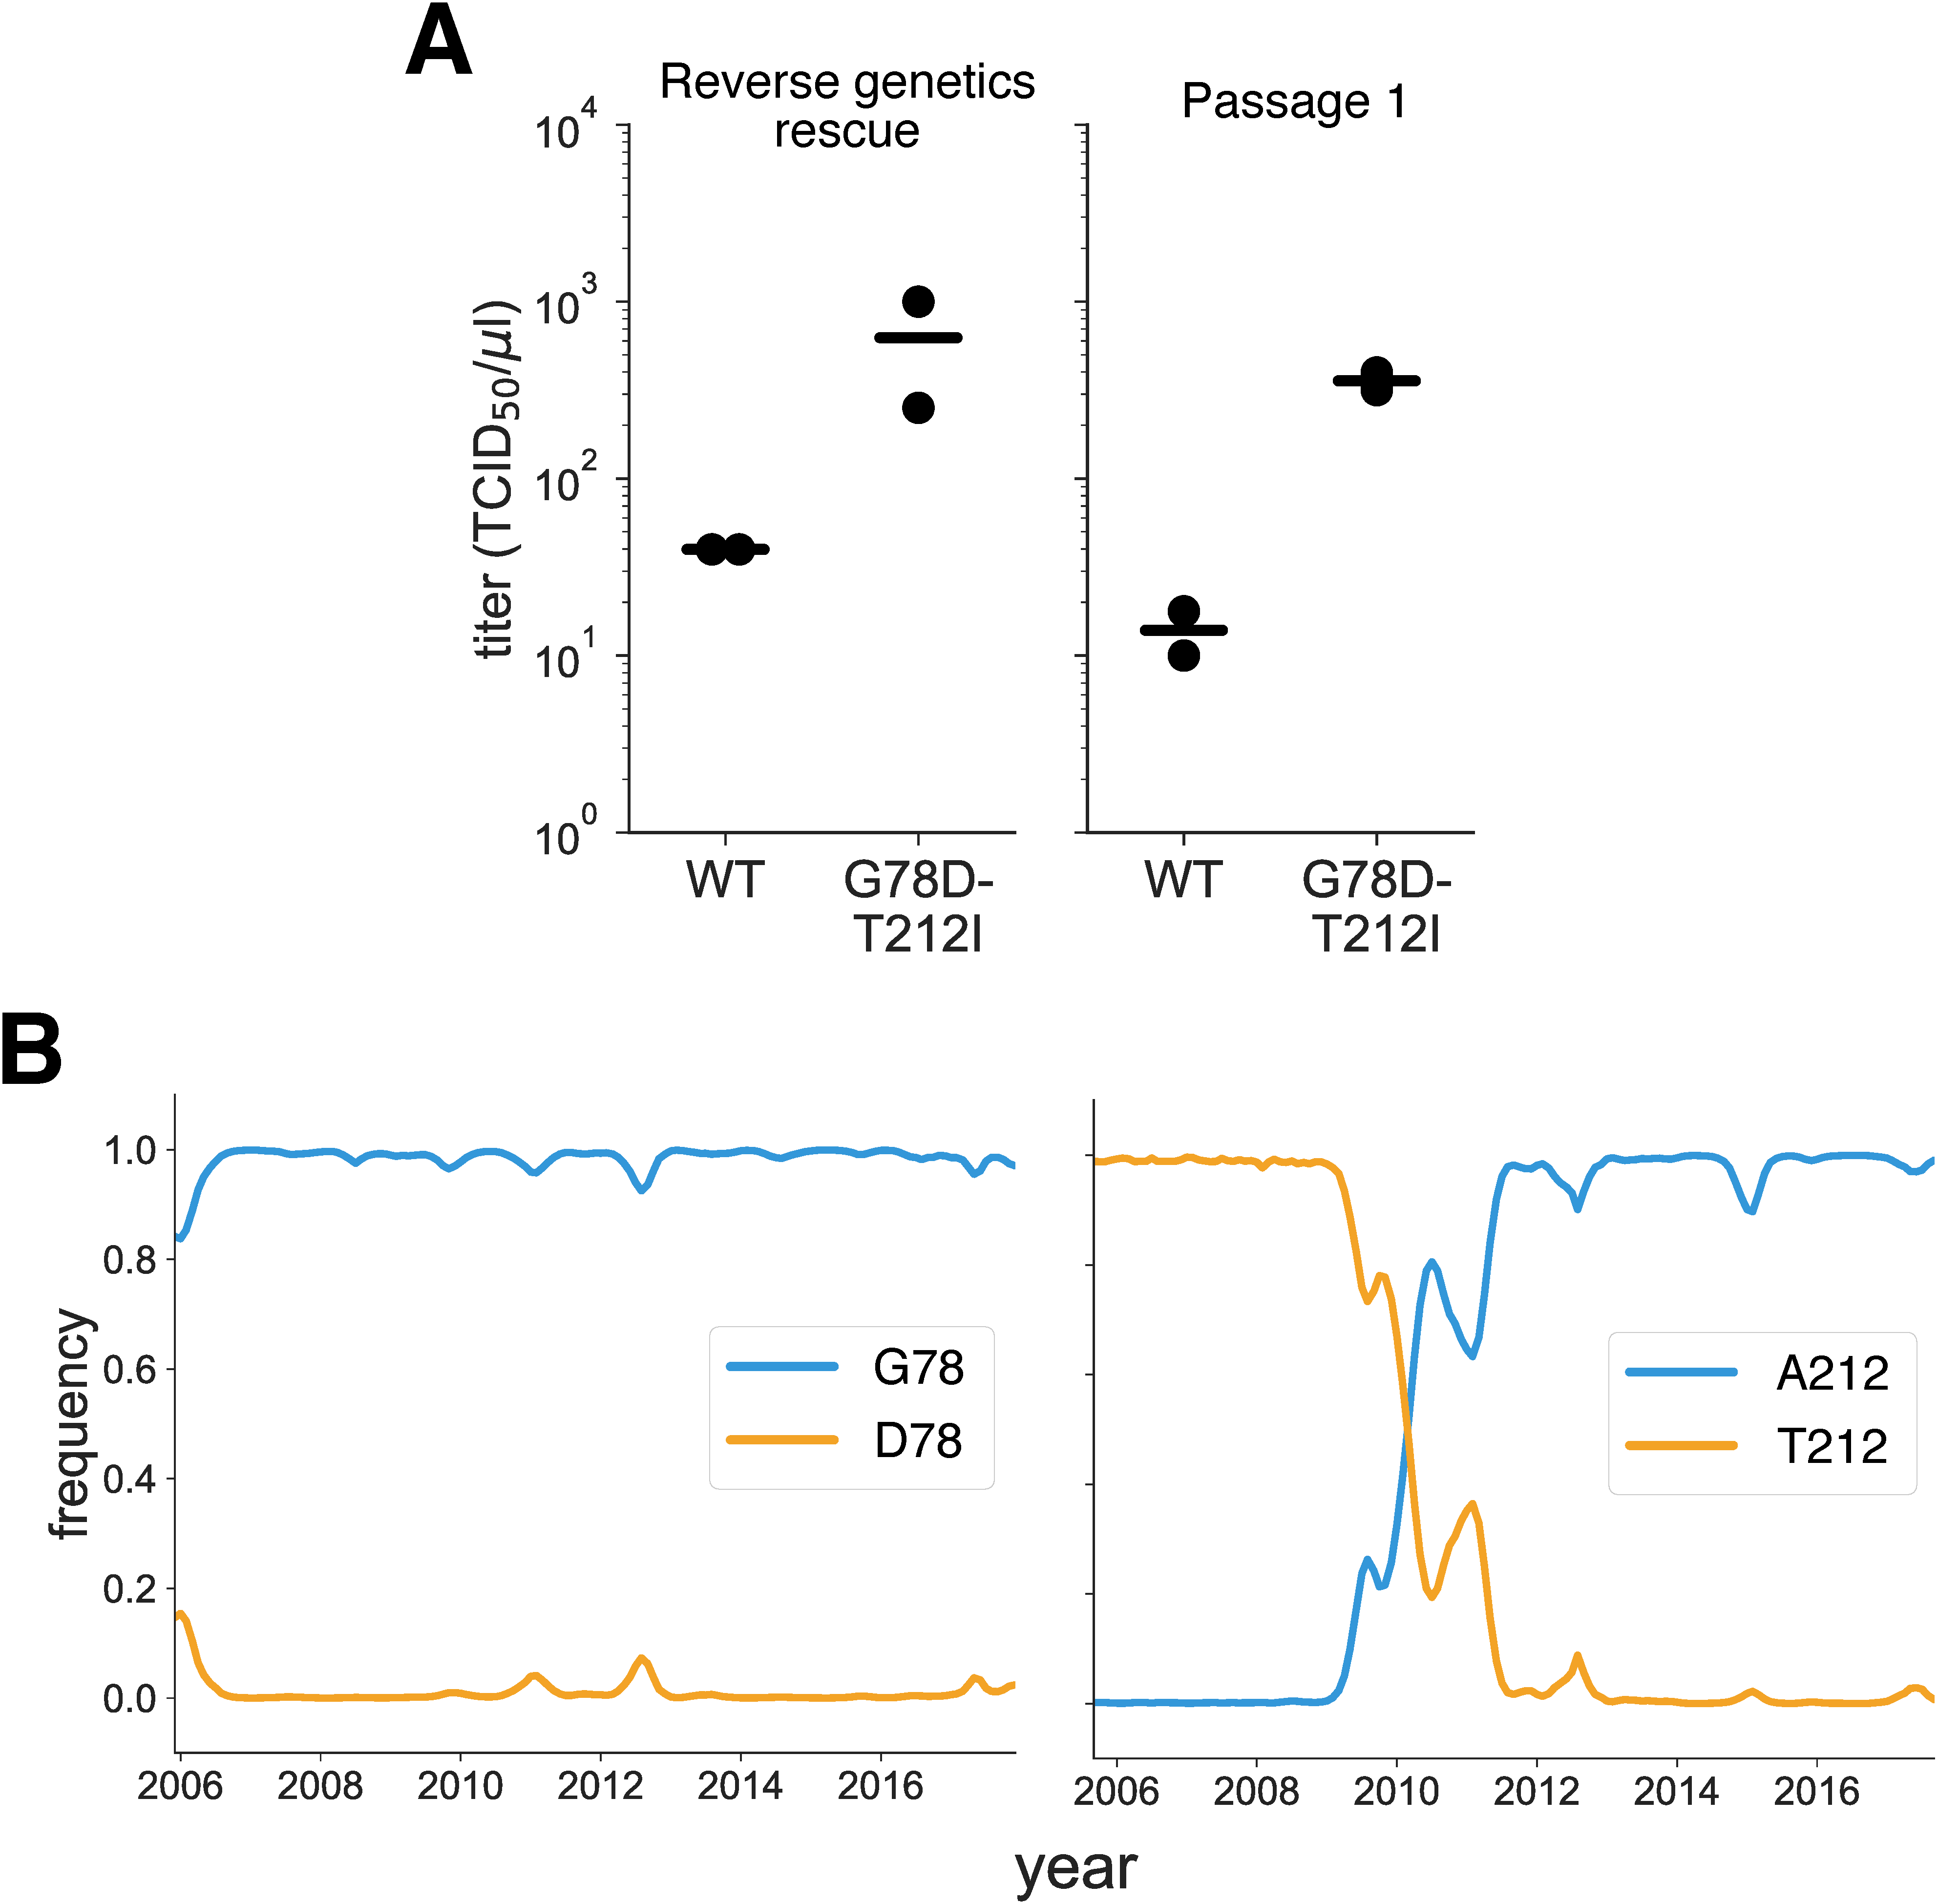
\includegraphics[width=0.5\textwidth]{figs/S01_G78D-T212I/G78D-T212I.pdf}}
\caption{\label{suppfig:Perth2009_mut}
{\bf Characterization of the G78D-T212I Perth/2009 HA variant.} 
(A) 
The G78D-T212I Perth/2009 HA variant supports better viral growth than the wildtype Perth/2009 HA.
Viruses were generated in duplicate by reverse genetics with the Perth/2009 NA and WSN internal genes, and passaged once at MOI = 0.01 in MDCK-SIAT1-TMPRSS2 cells.
The rescue and passage viral supernatants were collected at 72 hours post-transfection and 44 hours post-infection, respectively, and titered in MDCK-SIAT1-TMPRSS2 cells. 
The points mark each duplicate and the bar marks the mean.
(B)
The D78 variant remained at a low frequency in natural human H3N2 sequences over the past $~\sim$10 years.
The A212 variant rose to fixation in $~\sim$2011, replacing the T212 variant.
}
\end{suppfigure}

\begin{suppfigure}
\centerline{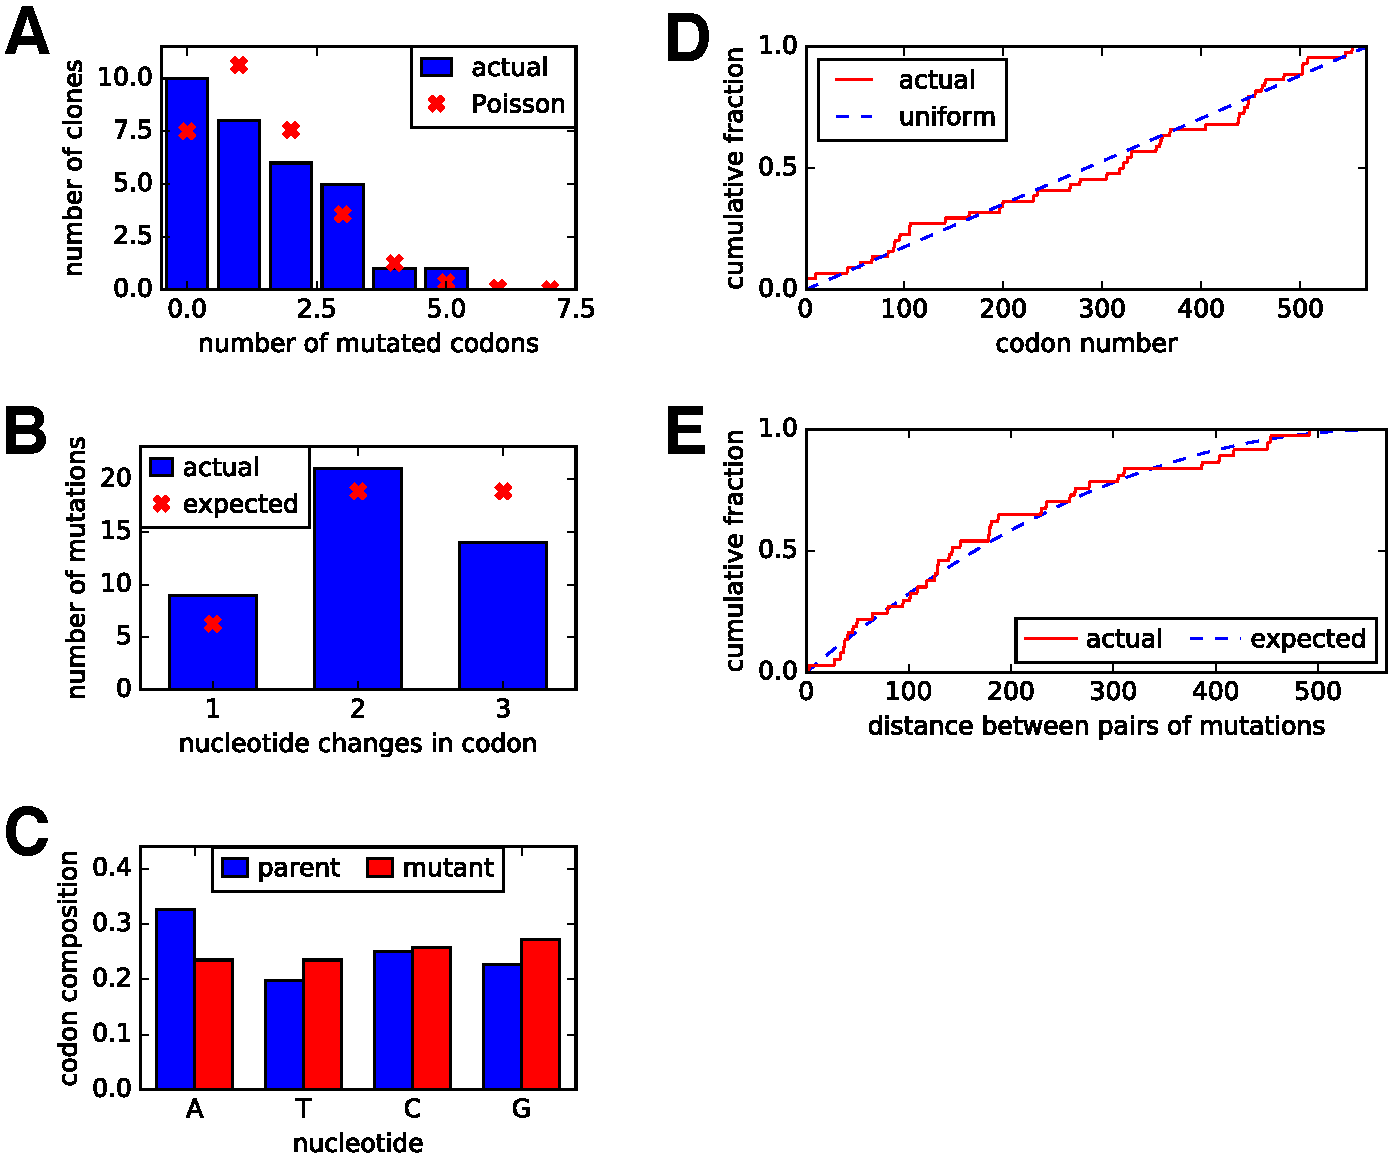
\includegraphics[width=0.6\textwidth]{figs/S02_SangerSeq/SangerSeq.pdf}}
\caption{\label{suppfig:SangerSeq}
{\bf Sanger sequencing of 31 randomly chosen clones from the mutant plasmid libraries.} 
(A) There were an average of $\sim$1.4 codon mutations per clone across the three plasmid mutant libraries.
(B) A mixture of one-, two-, and three-nucleotide mutations were present, with slightly fewer triple-nucleotide changes than expected.
(C) Nucleotide frequencies were uniform in the codon mutations.
(D) The mutations were distributed relatively evenly across the length of the HA coding sequence.
(E) We calculated the pairwise distances between mutations for clones carrying more than one mutation.
The cumulative distribution of these distances is shown in the red line. 
The blue line indicates the expected distribution if mutations in multiply mutated genes are randomly disbursed along the sequence. 
}
\end{suppfigure}

\begin{suppfigure}
\centerline{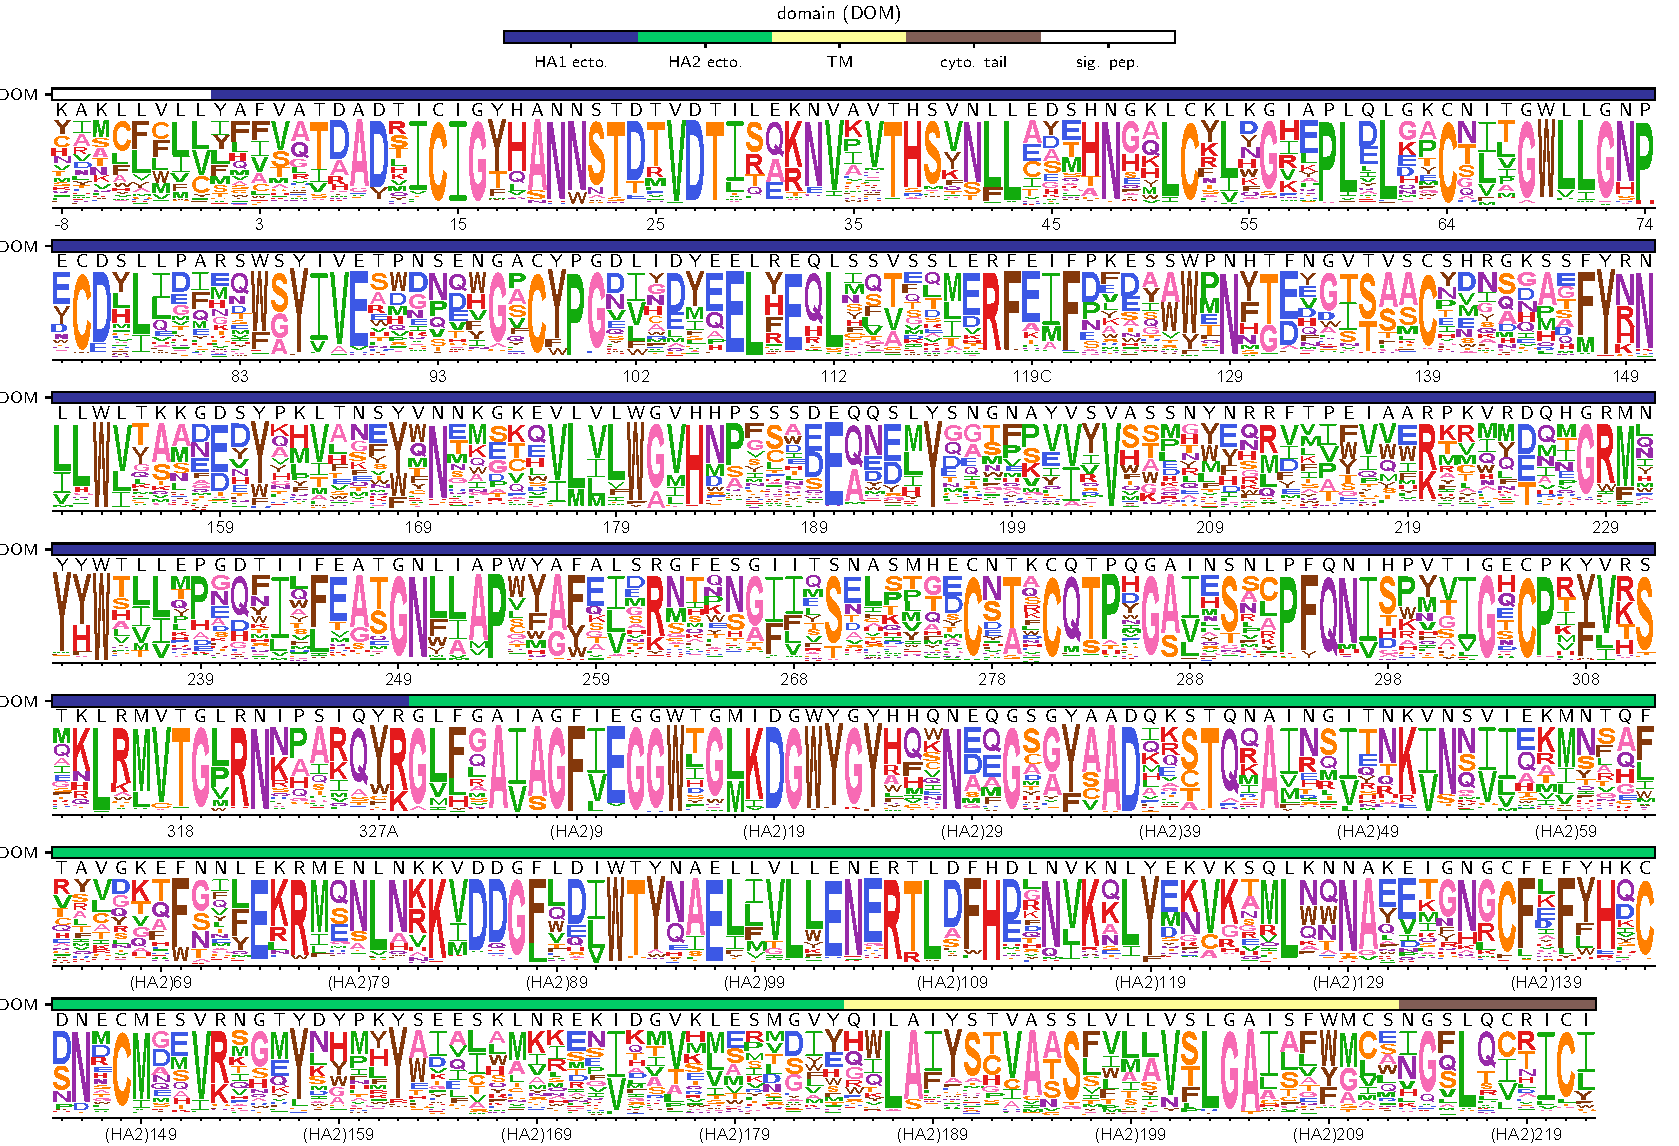
\includegraphics[width=\textwidth]{figs/S03_WSNprefs_logoplot/WSN-rescaled_prefs.pdf}}
\caption{\label{suppfig:WSNprefs_logoplot}
{\bf The site-specific amino-acid preferences of the WSN/1933 H1 HA.} 
The amino-acid preferences from~\cite{doud2016accurate} after taking the average of the experimental replicates and re-scaling~\cite{hilton2017phydms} by the stringency parameter \comment{somehow indicate where this stringency parameter}.
The sites are in H3 numbering.
\comment{I would suggest just getting rid of RSA. You might be able to replace the next two sentences by just saying: the overlays show the same information as in Figure X}.
The bottom overlay bar indicates the HA domain (sig. pep. = signal peptide, HA1 ecto. = HA1 ectodomain, HA2 ecto. = HA2 ectodomain, TM = transmembrane domain, cyto. tail. = cytoplasmic tail).
The letters directly above each logo stack indicate the wildtype amino acid at that site.
}
\end{suppfigure}

\begin{suppfigure}
\centerline{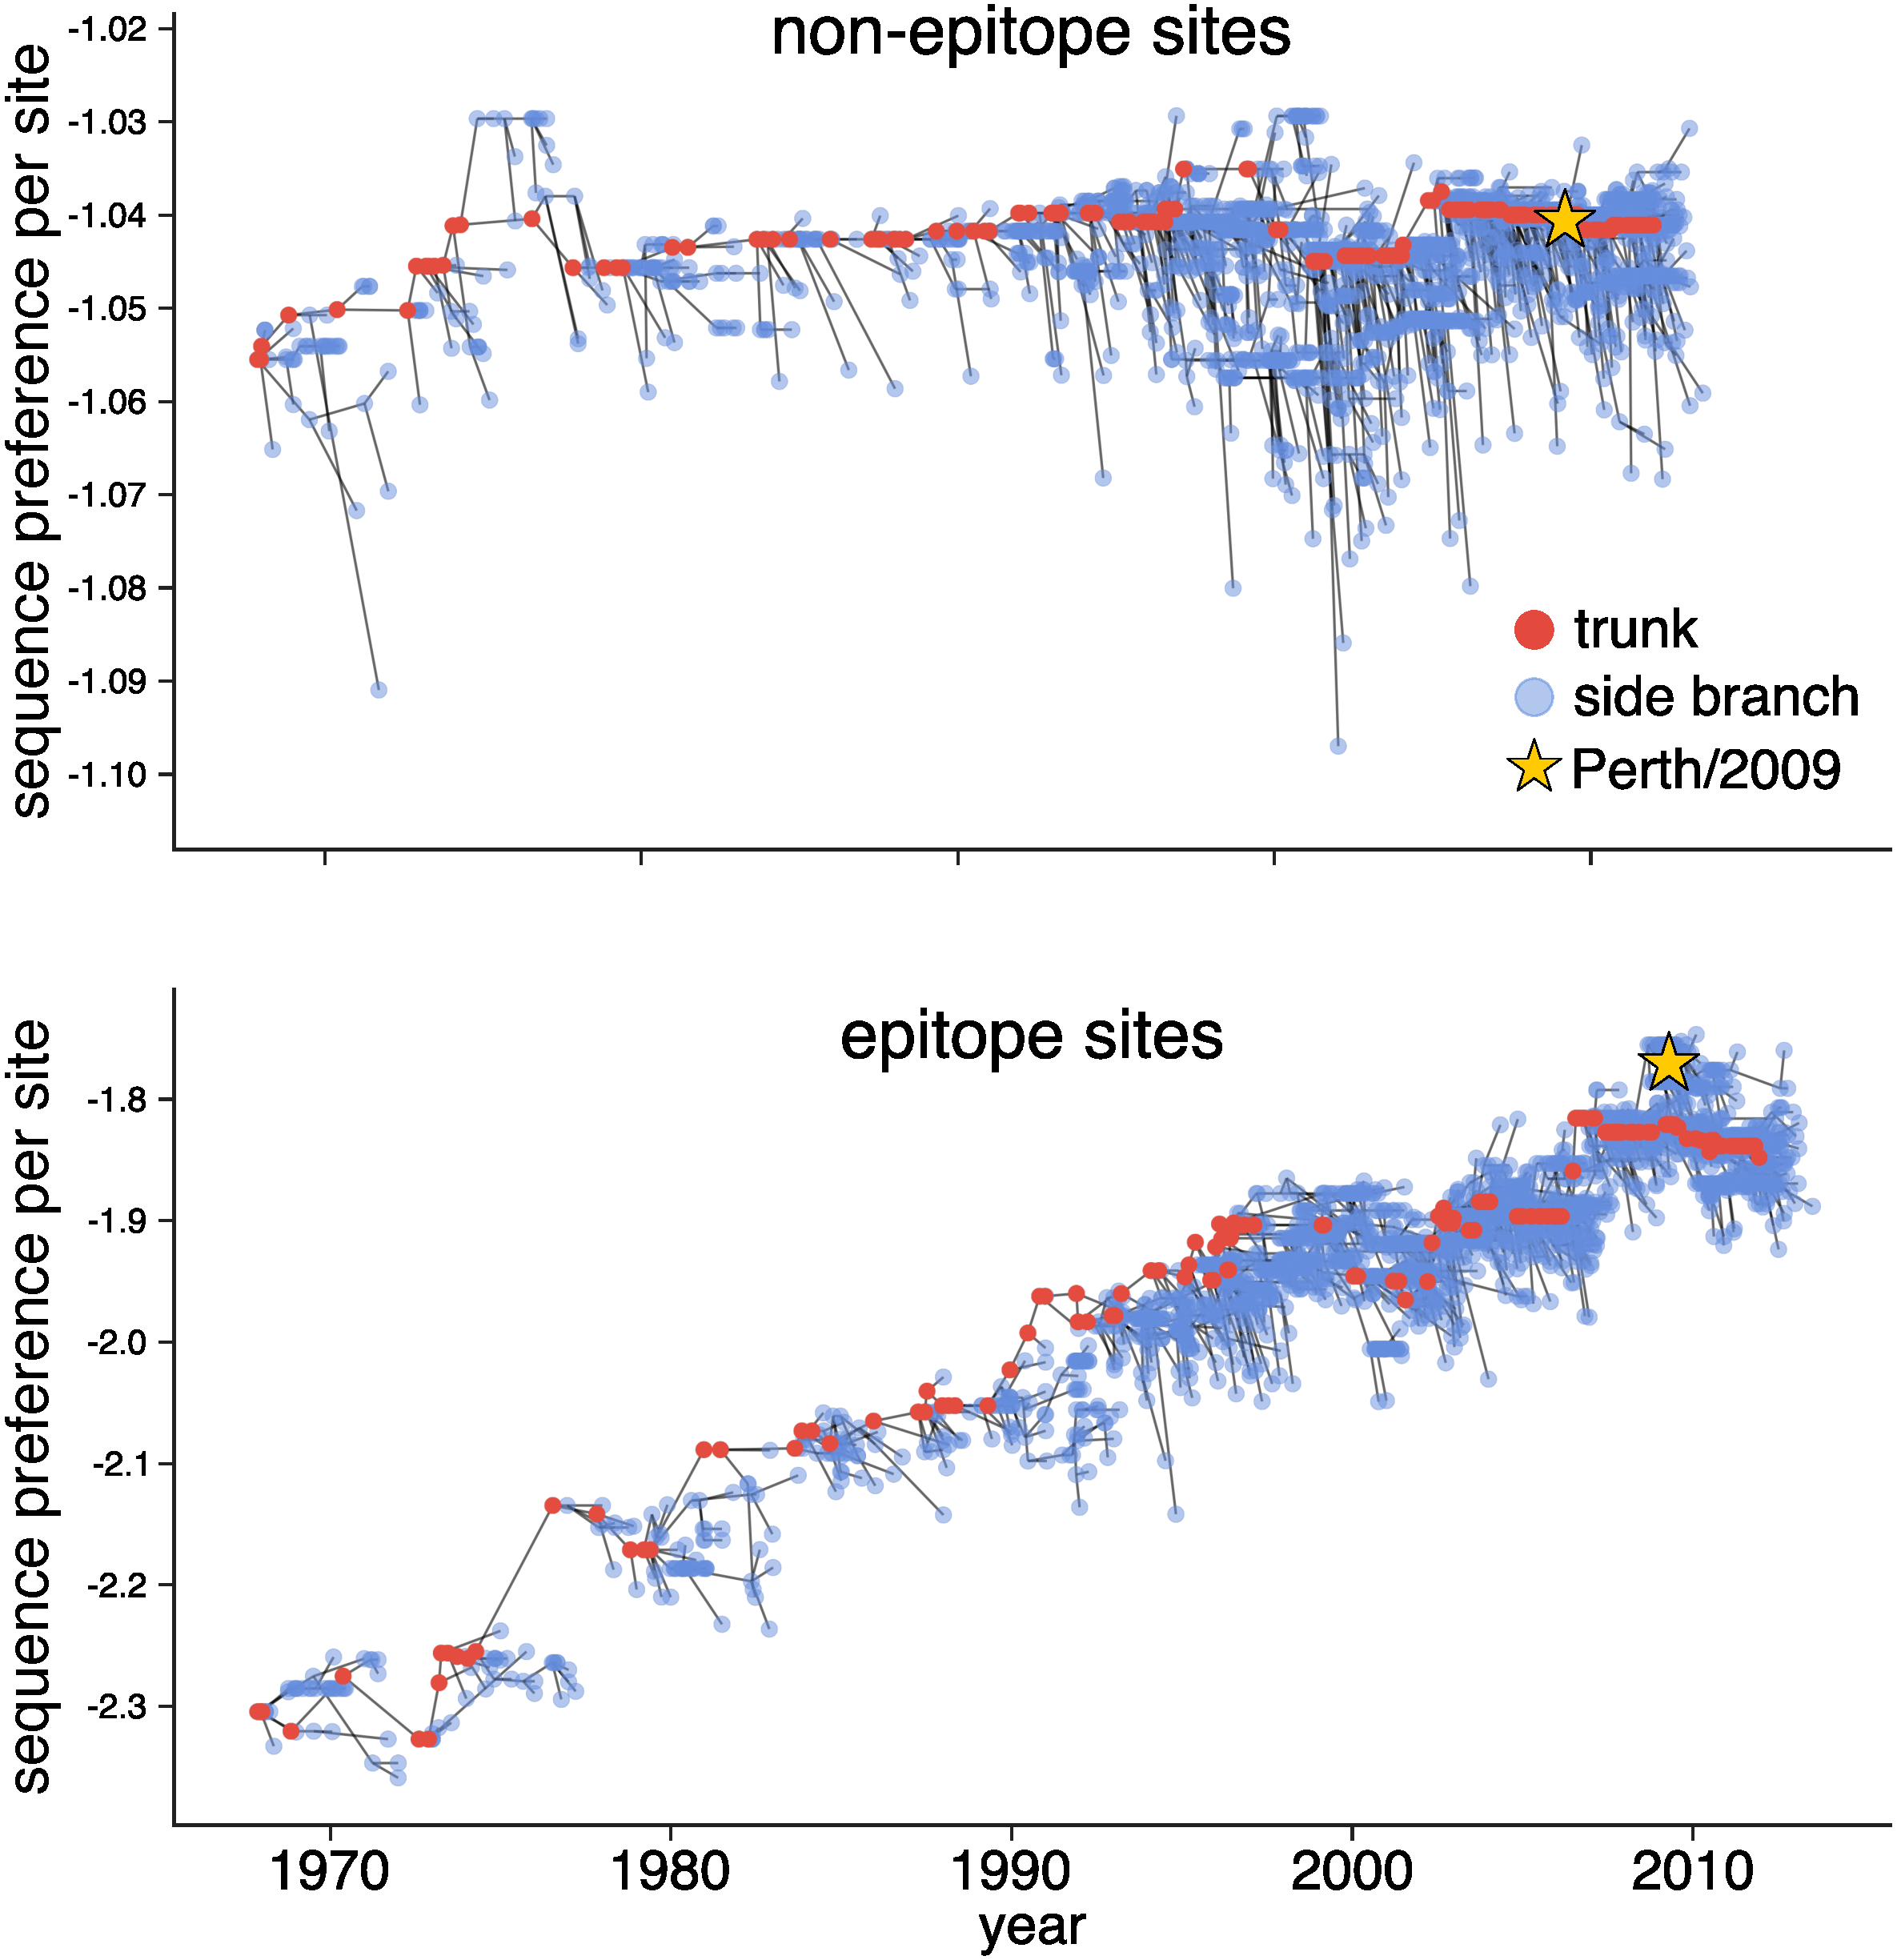
\includegraphics[width=0.6\textwidth]{figs/S04_seqpref_zoomed/seqpref_zoomed.pdf}}
\caption{\label{suppfig:seqpref_zoomed}
{\bf The per-site sequence preference at epitope and non-epitope sites}
The per-site sequence preferences shown in Figure~\ref{fig:sequence_preference}B, but on their own y-axes.
}
\end{suppfigure}

\subsubsection*{SI Tables}

Supply Word, RTF, or LaTeX files (LaTeX files must be accompanied by a PDF with the same file name for visual reference); include only one table per file. Do not use tabs or spaces to separate columns in Word tables.

\subsubsection*{SI Datasets} 

\begin{suppdata}
\caption{\label{suppdata:PerthHA}
Genbank file giving the full sequence of the bidirectional reverse-genetics plasmid pHW-Perth2009-HA-G78D-T212I, which encodes the wildtype HA sequence used in this study.
}
\end{suppdata}


\end{document}